% Chapter 4

\chapter{Desarrollo}
\label{capitulo4}

\index{Autenticación LTI|textit} \index{Ejecutar Código} \index{Editar Código} \index{Calificar Código} \index{Persistir Código} \index{Sincronizar Notas por LTI|textit} \index{Controlar Versiones de Código} \index{Recolección de Datos} \index{Toma de Decisiones}
\section{Preparaciones del Ambiente de Desarrollo}
Previo a realizar el desarrollo, es necesario que se prepara el ambiente para la misma con:
\begin{itemize}
  \item un sistema base (Debian Stretch con el Xen Hipervisor)
  \item un servidor local de Git (Git + Gitweb + NGinX),
  \item un servicio para recibir peticiones HTTP y convertirlos en sus respectivos objetos en un repositorio de Git (Git Server HTTP Endpoint)
  \item un LMS \index{LMS} (Moodle),
  \item un servidor de Git (GitLab CE)
  \item un servidor de Virtualización (Docker)
  \item plantillas de maquinas virtuales (en Docker)
\end{itemize}

\subsection{Sistema Base de Desarrollo}

\begin{figure}
	\begin{center}
    	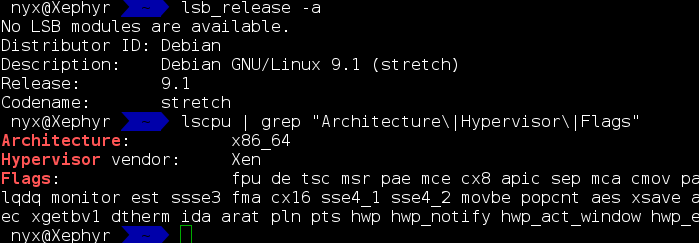
\includegraphics[width=0.75\textwidth]{Figures/sistema-base.png}
    \end{center}
  	\caption{Información del Sistema Base.}
    \label{sistema-base}
\end{figure}

\index{Ejecutar Código}
Como se presenta en la figura \ref{sistema-base}, el sistema base para el desarrollo de este trabajo de titulación utiliza Xen instalado con Debian Stretch (9.1)\footnote{Como el sistema de Dom0} instalado en un LVM con el nombre del grupo de volúmenes ''Xephyr-VG''. Originalmente se tenia planificado trabajar con Debian Jessie (8.x) debido que eso fue la versión estable al momento de instalación pero después se opto por una actualización a la versión beta de Debian en aquello momento (Debian Stretch). En resumen los pasos realizados fueron:
\lstset{language=Bash}
\begin{enumerate}
	\item Instalación Limpia de Debian 8 con un LVM.
    	\begin{description}
    		\item[Volumen Físico:] /dev/sda8 310g 
            \item[Grupo de Volúmenes:] Xephyr-VG 310g
            \item[Volúmenes Lógicos:] Originalmente 4 (se agrega 2 por cada nueva maquina virtual -- uno para su disco y otro para su área de intercambio).
            \begin{description}
            	\item[Xephyr-Dom0] Xephyr-VG 30g
                \item[Xephyr-IMG-Repo] Xephyr-VG 20g
                \item[Xephyr-ISO-Repo] Xephyr-VG 20g
                \item[Xephyr-Swap] Xephyr-VG 4g
            \end{description}
    	\end{description}
    \item Actualizar Instalación de Debian 8.
    	\begin{lstlisting}
	apt update
	apt upgrade
	apt dist-upgrade
	reboot
        \end{lstlisting}
    \item Actualizar Debian 8 a Debian 9.
        \begin{lstlisting}
	sed -i 's/jessie/stretch/g' /etc/apt/sources.list
	apt update
	apt upgrade
	reboot
        \end{lstlisting}
    \item Instalación de Herramientas de Trabajo
        \begin{lstlisting}
	apt install tmux vim zsh
        \end{lstlisting}
    \item Instalación y Configuración de Hipervisor Xen
		\begin{lstlisting}
	apt install xen-hypervisor
	dpkg-divert --divert /etc/grub.d/08_linux_xen \
		--rename /etc/grub.d/20_linux_xen
	update-grub
	cat > /etc/network/interfaces.d/xenbr << EOF

	auto xenbr0
	iface xenbr0 inet static
		address 10.10.10.1
		netmask 255.255.255.0
		bridge_ports wlan0

	#other possibly useful options in a
	#	virtualized environment
		#bridge_stp off		# disable
		#		Spanning Tree Protocol
		#bridge_waitport 0	# no delay
		#		before a port becomes
		#		available
		#bridge_fd 0		# no forwarding
		#		delay

	## configure a (separate) bridge for
	#	the DomUs without giving Dom0 an
	#	IP on it
	#auto xenbr1
	#iface xenbr1 inet manual
	#   bridge_ports eth1

	EOF

	reboot
		\end{lstlisting}
	\item Instalación de Herramientas de Xen
		\begin{lstlisting}
	apt install xen-tools xen-utils
		\end{lstlisting}
    \item Instalación de Herramientas de Desarrollo para Python 3
    	\begin{lstlisting}
	apt install python3 python3-virtualenv python3-pip
    	\end{lstlisting}
    \item Instalación de Servidores
    	\begin{lstlisting}
	apt install nginx-full postgresql mongodb\
    		redis-server gitweb fcgiwrap
    	\end{lstlisting}
    \item Instalación de Otros dependencias
        %  % TODO: Look for other possible dependencies?
    	\begin{lstlisting}
	apt install libffi-dev
    	\end{lstlisting}
    \item Instalación de IDEs en /opt. Se descargaron los respectivos .tar\textit{.xx} y se los descomprimieron en /opt con un comando similar al siguiente:
    	\begin{lstlisting}
	tar -axvf nombre.tar.xx -C\
    		/opt/ruta/raiz/donde/descomprimir
    	\end{lstlisting}
    \begin{enumerate}
    	\item PyCharm (Community o Professional Edition\footnote{Se ocupo una versión Professional, en parte por su buen suporte para desarrollo en Django) con una licencia estudiantil que actualmente es gratis de solicitar y renovar año tras año con un correo institucional})
        \item DBeaver (Community o Enterprise Edition\footnote{Históricamente siempre han sido gratis ambas versiones con la diferencia siendo que Enterprise Edition no es completamente software libre a diferencia de su versión libre, pero el mismo agrega suporte para bases de datos no relacionales. Se ocupo la versión Enterprise, entre los últimos ofertas gratis antes de que se convierte en un producto de pago, por este mismo motivo de requerir suporte para bases de datos NoSQL como MongoDB y Redis.})
    \end{enumerate}
\end{enumerate}

Estos pasos de instalación se basaron en la guía de instalación de Xen publicado en el wiki del proyecto de Debian \citep{Debian-Wiki-Xen}.

Para dar conexiones hace el exterior a las maquinas virtuales, se necesita activar una regla NAT en el cortafuego IPTables:

\begin{lstlisting}
	iptables -t nat -A POSTROUTING -o wlan0\
    		-j MASQUERADE
\end{lstlisting}

\index{Controlar Versiones de Código} \index{Persistir Código}
\subsubsection{Servidor Local de Git}
Para gestionar versiones de código escrito y facilitar la integración con sistemas externas y el sistema de virtualización, se levanta un servidor sencillo de Git.

Instalar paquetes para un interfaz web sencilla de Git:
\begin{lstlisting}
apt install git gitweb fcgiwrap
\end{lstlisting}

Se crea un usuario del sistema operativo solo para Git:
\begin{lstlisting}
adduser git
\end{lstlisting}

Se autentica como el usuario creado:
\begin{lstlisting}
su - git
\end{lstlisting}

Para tener repositorios ejemplares, se clona algunos repositorios:
\begin{lstlisting}
git clone --bare\
	https://gitlab.com/nishedcob/GitEDU.git\
	repositories/GitEDU.git
git clone --bare\
	https://gitlab.com/ArqAppGrpBravoEarleyVargas/\
    	GitEduERP.git\
	repositories/GitEduERP.git
\end{lstlisting}

Entrar al directorio de repositorios y arreglar permisos para permitir git push desde repositorios remotos:
\begin{lstlisting}
cd repositories/
for repo in `ls`; do
	cd $repo;
    pwd;
    chmod -R g+ws .;
    chgrp -R git .;
    git --bare update-server-info;
    cp hooks/post-update.sample hooks/post-update;
    chmod a+x hooks/post-update;
    cd ..;
done
\end{lstlisting}

Después se configura NGinX para trabajar con gitweb:
\begin{lstlisting}
# NGinX Config:
server {
        listen 80;
        listen [::]:80;
        server_name git.localhost 192.168.99.1 10.10.10.1;
        root /usr/share/gitweb;
        access_log /var/log/nginx/gitweb.access.log;
        # static repo files for cloning over https
        location ~ ^.*\.git/objects/([0-9a-f]+/[0-9a-f]+\
        	|pack/pack-[0-9a-f]+.(pack|idx))$ {
                root /home/git/repositories/;
        }

        # requests that need to go to git-http-backend
        location ~ ^.*\.git/(HEAD|info/refs|objects/info/.*\
        	|git-(upload|receive)-pack)$ {
                root /home/git/repositories;

                fastcgi_pass unix:/var/run/fcgiwrap.socket;
                fastcgi_param SCRIPT_FILENAME   /usr/lib/\
                	git-core/git-http-backend;
                fastcgi_param PATH_INFO          $uri;
                fastcgi_param GIT_PROJECT_ROOT  /home/git/\
                	repositories;
                fastcgi_param GIT_HTTP_EXPORT_ALL "";
                fastcgi_param REMOTE_USER $remote_user;
                include fastcgi_params;
        }

        # send anything else to gitweb if it's not a real file
        try_files $uri @gitweb;
        location @gitweb {
                fastcgi_pass unix:/var/run/fcgiwrap.socket;
                fastcgi_param SCRIPT_FILENAME   /usr/share/\
                	gitweb/gitweb.cgi;
                fastcgi_param PATH_INFO          $uri;
                fastcgi_param GITWEB_CONFIG      /etc/gitweb\
                	.conf;
                include fastcgi_params;
        }
}
\end{lstlisting}

Además se configura gitweb con la siguiente configuración:
\begin{lstlisting}
# Edit /etc/gitweb.conf
# path to git projects (<project>.git)
#$projectroot = "/var/lib/git";
$projectroot = "/home/git/repositories";
\end{lstlisting}

Prueba de que funciona:
\begin{lstlisting}
git clone http://git.localhost/nishedcob/GitEDU.git \
	GitEDU-test
\end{lstlisting}

Dado que el mismo GitWeb no tenga problemas con bajada de datos (\texttt{git fetch} / \texttt{git pull} / \texttt{git clone}) pero si tiene problemas con subida de datos como se lo require en EduNube para armar repositorios de ejecuccion validadas, se ve una necesidad de habilitar subida al mismo por SSH:

Como root en el servidor de Git, se cambia la clave del usuario de Git:
\begin{lstlisting}
passwd git
\end{lstlisting}

Como el usuario de EduNube en el servidor para el mismo:
\begin{lstlisting}
cd .ssh/
# Deja la llave generada sin clave:
ssh-keygen -f id_git
# Copia la llave publica al servidor
ssh-copy-id -i ~/.ssh/id_git.pub git@10.10.10.1
# Prueba que funciona
ssh -i ~/.ssh/id_git -vvv git@10.10.10.1
# Guardar la configuracion:
cat >> ~/.ssh/config < EOF

Host git
     HostName 10.10.10.1
     User git
     Port 22
     IdentityFile $HOME/.ssh/id_git

EOF
# Probar con:
ssh -vvv git
\end{lstlisting}

\index{Persistir Código} \index{Controlar Versiones de Código}
\subsubsection{Git Server HTTP Endpoint}
Para recibir llamadas HTTP y convertirlos en sus respectivos objetos en un repositorio de Git, se creó un miniservicio que realiza esta tarea, basado en la misma app de autenticación que utiliza EduNube:
\begin{lstlisting}
pipenv --three
pipenv install django six psycopg2 PyJWT bcrypt ipython \
	requests
pipenv run django-admin startproject GitServerHTTPEndpoint .
# Configurar Base de Datos, Reutilizar authApp de EduNube, \
#	migrar la base de datos, Crear un superusuario
rsync -av --progress ~/EduNube/authApp \
	~/GitServerHTTPEndpoint/
vim GitServerHTTPEndpoint/settings.py
pipenv run python manage.py makemigrations authApp
pipenv run python manage.py migrate
pipenv run python manage.py createsuperuser

pipenv run python manage.py runserver 8002
# crear un api token para GitEDU

pipenv run python manage.py startapp apiApp

pipenv lock --requirements | awk '{print $1}' > \
	requirements.txt
\end{lstlisting}

Se puede encontrar el repositorio para este servicio en \url{https://gitlab.com/nishedcob/GitServerHTTPEndpoint}.

\paragraph{Tokens de Autenticacion}
Para el uso del API del servicio de GitServerHTTPEndpoint, se emite tokens mediante un interfaz CRUD construido con formularios de Django. Esos API tokens son construidos bajo el estandar JWT o JSON Web Tokens donde el servidor (servicio de Django) generar una llave secreto (mediante la funcion generar sal de bcrypt) y con ello se cifra datos sobre el cliente con el fin de poder validar la identidad del mismo mediante el API token sin que el cliente puede modificar los datos de su API token. El mismo esquema de autenticacion para el API se utiliza con el servicio de EduNube. El acceso al mismo se puede encontrar en el url \url{http://10.10.10.1:8020/auth/tokens} y acceder con cualquier cuenta de superusuario para la creacion, lectura, actualizacion y eliminacion de los API Tokens.

\paragraph{API externa}
Los URLs del API de GitServerHTTPEndpoint toman la forma general de: 
\texttt{/api/<tipo\_de\_objeto>/<accion>/<ruta/de/objeto>}\\
donde los tipos de objetos posibles son
\begin{itemize}
	\item \texttt{ns} para los Namespace
    \item \texttt{repo} para Repositorios y
    \item \texttt{file} para Archivos
\end{itemize}
acciones posibles son:
\begin{itemize}
	\item \texttt{create} para crear,
	\item \texttt{edit} para editar y
    \item en el caso de los archivos, no existe un solo \texttt{edit} si no una subclasificacion de:
    \begin{itemize}
    	\item \texttt{edit/mv}
        para alterar la ruta de un archivo y 
        \item \texttt{edit/contents}
        para alterar los contenidos de un archivo.
    \end{itemize}
\end{itemize}

Los URIs del API que operan sobre Namespace, solo acceptan un namespace de parametro con un slash de delimitador final por ejemplo: \\
\texttt{/api/ns/create/nearley/}

Los URIs del API que opera sobre los repositorios requieren de parametros un namespace y repositorio igual con un slash de delimitador final por ejemplo: \\
\texttt{/api/repo/create/nearley/GitEDU/}

Los URIs del API que opera sobre archivos toman de parametros un namespace, un repositorio y una ruta de archivos que puede conllevar cualquier numero de slash para indicar directorios dentro del repositorio selecionado, pero la misma ruta no puede terminar en un slash, por ejemplo: \\
\texttt{/api/file/create/nearley/GitEDU/despliegue/Readme.md}

Un cliente ejemplar de todo el API, se puede encontrar con el nombre \\
\texttt{example\_client.py} dentro del raiz del proyecto.

\index{Sincronizar Notas por LTI} \index{Autenticación LTI}
\subsection{Ambiente Virtual de LMS \index{LMS} (Moodle)}
\label{instalacion-moodle}
Originalmente fue planteada trabajar con el LMS como una máquina virtual de Xen, pero con el tiempo, se ha visto una necesidad de consumir todos los servicios possibles de una forma mas liviana y por lo tanto aunque se incluye por este medio la instalación de Moodle en una máquina virtual de Xen, al final se optó por un levantamiento del mismo en Docker. El levantamento de Moodle en Docker se documenta en el capitulo \ref{capitulo6} de Despliegue.

\subsubsection{Maquina Virtual de Xen}
Para el ambiente de Moodle (LMS \index{LMS} contra el cual se ha llevado el desarrollo), se crea una maquina virtual de Debian Stretch (9) con 1 GiB de RAM, 1 CPU virtual, 6 GiB de disco, 512 MiB de intercambio y una dirección IP fija de 10.10.10.10. Los resultados del mismo comando se puede ver en la figura \ref{vm-moodle}.
\begin{lstlisting}
	xen-create-image --hostname=debian-moodle\
    		--ip=10.10.10.10 --netmask=255.255.255.0\
        	--gateway=10.10.10.1 --memory=1024mb\
        	--vcpus=1 --lvm=Xephyr-VG --pygrub\
        	--dist=stretch --force --size=6144mb\
        	--swap=512mb
\end{lstlisting}

\begin{figure}
	\begin{center}
    	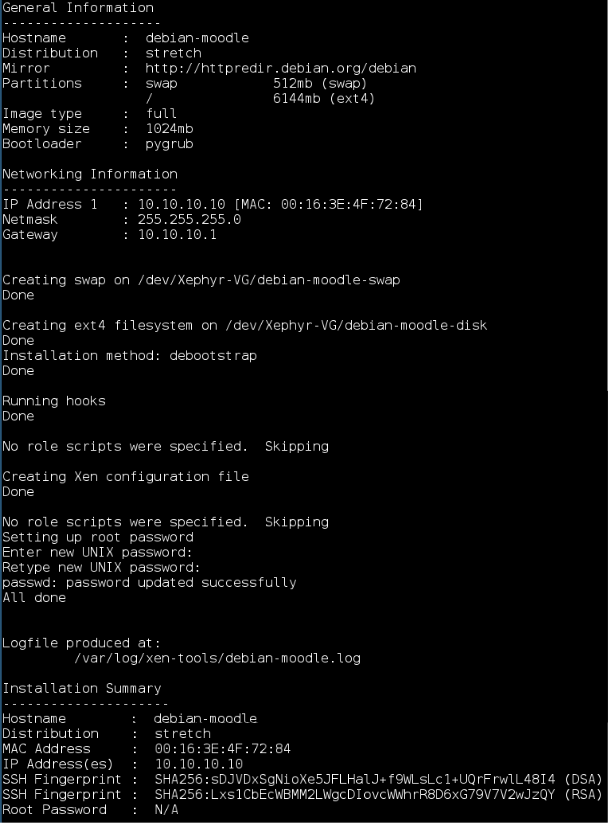
\includegraphics[width=0.75\textwidth]{Figures/crear-moodle.png}
    \end{center}
  	\caption{Crear maquina virtual para Moodle.}
    \label{vm-moodle}
\end{figure}

Se renombró el archivo de configuración de la maquina virtual generado en el paso anterior para temas de consistencia.

\begin{lstlisting}
	mv /etc/xen/debian-moodle.cfg\
    		/etc/xen/domU-debian-moodle.cfg
\end{lstlisting}

Un bug de Xen-Tools causa que no se instala correctamente un núcleo de Linux en la maquina virtual y por lo tanto es necesario entrar al mismo con un Chroot y instalar los paquetes faltantes (y hacer las adecuadas configuraciones  para permitir su arranque independiente de ayuda externa).

\begin{lstlisting}
	mount /dev/Xephyr-VG/debian-moodle-disk /mnt
	mount -o bind /proc /mnt/proc
	mount -o bind /sys /mnt/sys
	mount -o bind /dev /mnt/dev
	cp /etc/resolv.conf /mnt/etc/resolv.conf
	chroot /mnt /bin/bash
	apt install linux-image-amd64
	vim.tiny /boot/grub/menu.lst
	# Revisar que los archivos referenciados existen
	#		de verdad por ejemplo:
	# Replace initrd.img- con initrd.img
    # guarda y sale
	exit
	umount /mnt/proc            
	umount /mnt/sys 
	umount /mnt/dev 
	umount /mnt	
\end{lstlisting}

Para levantar la maquina virtual:

\begin{lstlisting}
	xl create /etc/xen/domU-debian-moodle.cfg -c
\end{lstlisting}

Se debe seleccionar la tercera opción (Default Kernel).

Se puede dar una revisión a la configuración de red para asegurarse de que esta correcto:

\begin{lstlisting}
	vim.tiny /etc/network/interfaces
\end{lstlisting}

Debe contener:

\begin{lstlisting}
auto eth0
iface eth0 inet static
 address 10.10.10.10
 gateway 10.10.10.1
 netmask 255.255.255.0
\end{lstlisting}

En el presente caso, Xen-Tools logró configurar esta parte de forma correcta.

A continuación se procede con la instalación de Moodle:

\begin{lstlisting}
# actualiza el sistema
apt update
apt upgrade

# instala dependencias
apt install apache2 php7.0 mysql-server php7.0-mysql
apt install libapache2-mod-php7.0 php7.0-gd php7.0-curl
apt install php-xml php-zip php-mbstring php-soap
apt install php7.0-xmlrpc php7.0-intl
vim.tiny /etc/php/7.0/apache2/php.ini

# agrega:
extension=mysql.so 
extension=gd.so

# edita:

memory_limit = 40M
# dejado con el valor por defecto de 128M

post_max_size = 80M
upload_max_filesize = 80M

# guarda y sale

# reinicia apache para coger los cambios
systemctl restart apache2

\end{lstlisting}

A continuación se configura la base de datos:

\begin{lstlisting}

# clave de root es root
mysqladmin -u root password "root"

# iniciar session como root
mysql -u root -p

# crear base de datos y hacer que ocupa UTF-8
mysql> CREATE DATABASE moodle;
mysql> ALTER DATABASE moodle charset=utf8;
mysql> exit;

## No se implemento ##
# Moodle queja de UTF8

# Se podria arreglar
# (antes de instalar Moodle)
# con:

mysql -u root -p

mysql> ALTER DATABASE moodle charset=utf8mb4;
mysql> exit;
######################

systemctl restart mysql

\end{lstlisting}

Se realiza la instalación de la ultima versión de Moodle (3.3 con sus respectivos patches de fallas desde que el mismo salio):

\begin{lstlisting}

# descargar
wget https://download.moodle.org/download.php/direct/stable33/\
	moodle-latest-33.tgz

# descomprimir
tar -zxvf moodle-latest-33.tgz

# meter en la ubicacion para apache
mv moodle /var/www

# ir a ubicacion para apache
cd /var/www

# crear ubicacion para datos
mkdir moodledata

# arreglar permisos
chown -R www-data:www-data moodle
chown -R www-data:www-data moodledata
chmod -R 755 moodle
chmod -R 755 moodledata

# modificar configuracion de apache
vim.tiny /etc/apache2/sites-available/000-default.conf

# editar
DocumentRoot "/var/www/moodle"

# guardar y salir

# reiniciar apache para aplicar los cambios
systemctl restart apache2

\end{lstlisting}

Arreglar la base de datos para que acepte conexiones desde Moodle:

\begin{lstlisting}

mysql -u root -p

GRANT ALL PRIVILEGES on *.* to
	'root'@'localhost' IDENTIFIED BY 'root';
GRANT ALL PRIVILEGES on *.* to
	'root'@'localhost' IDENTIFIED BY 'root';
FLUSH PRIVILEGES;
exit;

\end{lstlisting}

Para seguir con la instalación se abre un navegador con la dirección \url{http://10.10.10.10/} para seguir las instrucciones que se le lleve por toda la configuración inicial del Moodle.

Al final se agregue un trabajo de cron para ayudar con los tareas periódicas que Moodle requiere para su mantenimiento continuo:

\begin{lstlisting}

crontab -u www-data -e
# add line:
*/10 * * * * /usr/bin/php
		/var/www/moodle/admin/cli/cron.php
        		>/dev/null

\end{lstlisting}

Estos pasos fueron adaptados de la guía oficial del proyecto de Moodle para instalación en Debian \citep{MOODLE-Install-Debian}.

Ahora que todo esta funcionando se recomienda editar /boot/grub/menu.lst para comentar las entradas del pyGrub que son defectuosas (los primeros dos) para que se puede levantar la maquina virtual sin intervención humana.

\index{Persistir Código} \index{Controlar Versiones de Código}
\subsection{Servidor de Git (GitLab CE)}
Originalmente fue planteada trabajar con GitLab Community Edition como una máquina virtual de Xen, pero con el tiempo, se ha visto una necesidad de consumir todos los servicios possibles de una forma mas liviana y por lo tanto aunque se incluye por este medio la instalación del mismo en una máquina virtual de Xen, al final se optó por un levantamiento del mismo en Docker. El levantamento de GitLab en Docker se documenta en el capitulo \ref{capitulo6} de Despliegue.

\subsubsection{Máquina Virtual de Xen}
Para crear el servidor de Git con GitLab Community Edition, se va a empezar con las mismas piezas del servidor del LMS/Moodle, es decir una maquina virtual de Debian 9. El mismo se crea como una maquina virtual de Debian Stretch (9) con 1 GiB de RAM, 1 CPU virtual, 6 GiB de disco, 512 MiB de intercambio y una dirección IP fija de 10.10.10.11.
\begin{lstlisting}
	xen-create-image --hostname=debian-gitlab\
    		--ip=10.10.10.11 --netmask=255.255.255.0\
        	--gateway=10.10.10.1 --memory=1024mb\
        	--vcpus=1 --lvm=Xephyr-VG --pygrub\
        	--dist=stretch --force --size=6144mb\
        	--swap=512mb
\end{lstlisting}

Se renombró el archivo de configuración de la maquina virtual generado en el paso anterior para temas de consistencia.

\begin{lstlisting}
	mv /etc/xen/debian-gitlab.cfg\
    		/etc/xen/domU-debian-gitlab.cfg
\end{lstlisting}

Un bug de Xen-Tools causa que no se instala correctamente un núcleo de Linux en la maquina virtual y por lo tanto es necesario entrar al mismo con un Chroot y instalar los paquetes faltantes (y hacer las adecuadas configuraciones  para permitir su arranque independiente de ayuda externa).

\begin{lstlisting}
	mount /dev/Xephyr-VG/debian-gitlab-disk /mnt
	mount -o bind /proc /mnt/proc
	mount -o bind /sys /mnt/sys
	mount -o bind /dev /mnt/dev
	cp /etc/resolv.conf /mnt/etc/resolv.conf
	chroot /mnt /bin/bash
	apt install linux-image-amd64
	vim.tiny /boot/grub/menu.lst
	# Revisar que los archivos referenciados existen
	#		de verdad por ejemplo:
	# Replace initrd.img- con initrd.img
    # guarda y sale
	exit
	umount /mnt/proc            
	umount /mnt/sys 
	umount /mnt/dev 
	umount /mnt	
\end{lstlisting}

Para levantar la maquina virtual:

\begin{lstlisting}
	xl create /etc/xen/domU-debian-gitlab.cfg -c
\end{lstlisting}

Se debe seleccionar la tercera opción (Default Kernel).

Se puede dar una revisión a la configuración de red para asegurarse de que esta correcto:

\begin{lstlisting}
	vim.tiny /etc/network/interfaces
\end{lstlisting}

Debe contener:

\begin{lstlisting}
auto eth0
iface eth0 inet static
 address 10.10.10.11
 gateway 10.10.10.1
 netmask 255.255.255.0
\end{lstlisting}

En el presente caso, Xen-Tools logró configurar esta parte de forma correcta.

A continuación se procede con la instalación de Gitlab:

\begin{lstlisting}
# actualiza el sistema
apt update
apt upgrade

# A partir del Debian 9, Gitlab CE esta ofrecido
#    en los repositorios oficiales:
apt install gitlab

# Arreglar problema con API
vim.tiny /usr/share/gitlab-shell/config.yml
# cambiar gitlab_url a "http://10.10.10.11/"

/usr/share/gitlab-shell/bin/check
\end{lstlisting}

Visitar \url{http://10.10.10.11/} y configurar la contraseña del usuario root. Con el usuario root configurado se procede a crear un usuario especial para la aplicación con el nombre de usuario 'GitEdu'. Este usuario lo damos permisos de administración y también se genera un token en esta dirección: \url{http://10.10.10.11/profile/personal_access_tokens}. El token se debe guardar para su uso después (GitLab nunca le vuelve a mostrar).

Ahora que todo esta funcionando se recomienda editar /boot/grub/menu.lst para comentar las entradas del pyGrub que son defectuosas (los primeros dos) para que se puede levantar la maquina virtual sin intervención humana.

\index{Ejecutar Código}
\subsection{Servidor de Virtualización}
Para la ejecución de código se considera necesario la virtualización. La ejecución puramente nativa de código daría mayor superficie de ataque al servidor físico además de no permitir mayor flexibilidad necesaria para sostener una gran variedad de usuarios y necesidades.

\index{Ejecutar Código}
\subsubsection{Comparación de Hipervisores}
Para la selección de una tecnología de virtualización, se ha considerado conveniente realizar el siguiente cuadro comparativo en base a una valoración de características de cada ecosistema de hipervisor para generar una calificación ponderada de las mismas y poder llegar objetivamente al mejor hipervisor a ser implementado en el presente proyecto.

\begin{table}
	\centering
	\begin{tabular}{|l|r|}
    	\hline
		\textbf{Característica} & \textbf{Peso} \\
        \hline
        \textit{Rendimiento} & 10 \\
        \textit{Seguridad} & 10 \\
        \textit{Facilidad de Uso (CLI)} & 10 \\
        \textit{Facilidad de Uso (GUI)} & 5 \\
        \textit{Facilidad de Uso (WUI)} & 5 \\
        \textit{Facilidad de Instalación} & 5 \\
        \textit{Facilidad de Mantenimiento} & 5 \\
        \textit{Experiencia Personal del Autor} & 10 \\
        \hline
        \textbf{Total de Pesos} & 60 \\
        \hline
	\end{tabular}
    \caption{Pesos de las Características de Comparación para Hipervisores Considerados}
    \label{tab:hipervisor-compar-pesos}
\index{Ejecutar Código}
\end{table}

El cuadro \ref{tab:hipervisor-compar-pesos} presenta las pesos que se asignaron a cada categoría de la comparación para poder realizar un promedio ponderado de las valoraciones con mayor peso en las categorías que se consideraban más importantes. Las características consideradas son:
\begin{description}
	\item[Rendimiento] Indica la máxima eficiencia que puede llegar a tener la virtualización con esta tecnología.
    \item[Seguridad] Indica el nivel de aislamiento y mitigación de riesgo que se considera los usuarios virtualizados frente la maquina host.
    \item[Facilidad de Uso (CLI)] La facilidad en utilizar el hipervisor desde linea de comandos (terminal).
    \item[Facilidad de Uso (GUI)] La facilidad en utilizar el hipervisor desde aplicación de escritorio gráfica.
    \item[Facilidad de Uso (WUI)] La facilidad en utilizar el hipervisor desde plataforma web.
    \item[Facilidad de Instalación] La facilidad para instalar el hipervisor y realizar la configuración inicial para que empieza a funcionar.
    \item[Facilidad de Mantenimiento] La facilidad para actualizar, utilizar y mantener el hipervisor.
    \item[Experiencia Personal del Autor] La opinión tiene el autor del hipervisor después de años de uso y experimentación en estas tecnologías.
\end{description}
Se ha considerado con mayor importancia el Rendimiento y la Seguridad como necesidades del presente proyecto. La Facilidad de Uso desde Línea de Comandos y la Experiencia Personal del Autor también se ha considerado importante para que se pueda implementar de forma mas concisa, rápida y precisa la tecnología de virtualización elegida. La Facilidad de Uso tanto Gráfica como Web en adición a la complejidad de Instalación y Mantenimiento se considera importantes pero menos relevantes debido a que son características de menor impacto para el desarrollo actual y al largo plazo donde tienen mayor impacto se puede implementar otra solución mas adecuada frente esos temas si es necesario. 

\begin{table}
	\centering
	\begin{tabular}{|p{1.85cm}|p{2.25cm}|p{1.8cm}|p{1.7cm}|p{1.7cm}|p{1.7cm}|}
    	\hline
		\textbf{Hipervisor} & \textbf{Rendimiento} & \textbf{Seguridad} & \textbf{Facilidad de Uso (CLI)} & \textbf{Facilidad de Uso (GUI)} & \textbf{Facilidad de Uso (WUI)} \\
        \hline
        \textit{Xen} & 4 & 5 & 4 & 3 & 2 \\
        \hline
        \textit{KVM} & 3 & 5 & 4 & 3 & 3 \\
        \hline
        \textit{Docker} & 5 & 3 & 5 & 3 & 4 \\
        \hline
	\end{tabular}
    \caption{Características de Comparación I: Hipervisores Considerados}
\index{Ejecutar Código}
    \label{tab:hipervisor-compar-i}
\end{table}

\begin{table}
	\centering
	\begin{tabular}{|p{1.85cm}|p{2.2cm}|p{3.0cm}|p{1.9cm}|}
    	\hline
		\textbf{Hipervisor} & \textbf{Facilidad de Instalación} & \textbf{Facilidad de Mantenimiento} & \textbf{Experiencia Personal del Autor} \\
        \hline
        \textit{Xen} & 3 & 2 & 4 \\
        \hline
        \textit{KVM} & 4 & 2 & 2 \\
        \hline
        \textit{Docker} & 5 & 4 & 4 \\
        \hline
	\end{tabular}
    \caption{Características de Comparación II: Hipervisores Considerados}
\index{Ejecutar Código}
    \label{tab:hipervisor-compar-ii}
\end{table}

% TODO: Correccion de la Maria del Carmen "caracteristicas consideradas"?
En los cuadros \ref{tab:hipervisor-compar-i} y \ref{tab:hipervisor-compar-ii} se presenta las características consideras y un puntaje relativo (sobre 5) dada a cada una de las mismas según las investigaciones, experiencias y opiniones del autor. A continuación se explica el porque de las valoraciones:
\begin{description}
	\item[Xen] como un hipervisor de tipo uno se cuenta con un rendimiento muy alto, especialmente cuando se toma en cuenta la paravirtualización que también se suporta con sistemas operativos modificados, casi a un nivel nativo. Este hipervisor logra virtualizar todas las capas de un sistema operativo, desde su núcleo hasta el espacio de los usuarios, pero al mismo tiempo dispone de un modelo de seguridad muy buena. Falla en las herramientas de administración de los cuales hay muy pocas que están actualizadas. La mejor herramienta de administración es en la Línea de Comandos. Sus cambios frecuentes y documentación desactualizada son un problema para la instalación y mantenimiento. La experiencia del autor con esta tecnología ha sido muy positiva.
    \item[KVM] como un hipervisor de tipo uno y medio es más alto nivel que Xen y no dispone del mismo nivel de rendimiento que ofrece ni la paravirtualización. Aunque es más alto nivel, se ha tomado pasos adicionales para que alcanza un nivel de seguridad equivalente a la de Xen. Para su administración cuenta con herramientas muy similares a los de Xen, pero su alto nivel de integración con el API de Libvirt hace que puente con mejores interfaces para su manejo web. Posiblemente por desconocimiento de las posibilidades para mejorar el rendimiento que se puede aplicar, el autor no ha tenido una experiencia muy positiva con la aplicación de esta tecnología de virtualización.
    \item[Docker] como un hipervisor de ''tipo tres'' es de muy alto nivel y dispone de una seguridad mucho menor al tener menor aislamiento entre el sistema que provee la virtualización y la virtualizada. Docker tiene mejor rendimiento ya que se virtualiza solo los niveles más altos de un sistema operativo y las aplicaciones que se encuentran por encima. Su técnica de containerización como un tipo de virtualización que puede dar mejor rendimiento que la paravirtualización. Se considera muy buena las interfaces para utilizar Docker, tanto a nivel de terminal como a nivel web. Puede que sea el caso por el hecho de que Docker es una tecnología que aún es bastante nueva y que esta en auge. Esto promueve una gran cantidad de personas a estar contribuyendo sus mejoras. La instalación y mantenimiento de Docker es muy sencillo en cualquier plataforma. Debido a su sencillez, alto rendimiento, funcionalidad y utilidad, el autor ha tenido una buena experiencia con el uso de esta tecnología de virtualización. 
\end{description}

Para calcular los pesos promediados de forma ponderada se aplica la siguiente formula que se encuentra en la figura \ref{fig:hipervisor-calif-equ}. Las calificaciones promedias se reflejan en el cuadro \ref{tab:hipervisor-compar-promed}. Como se puede observar del mismo cuadro, frente los criterios previamente establecidos, Docker se puede considerar la mejor tecnología de virtualización en el proyecto actual con un puntaje de $4.167$, con medio punto mas que su competencia mas cercana Xen, $3.667$ y $\frac{5}{6}$ de un punto mas que KVM, $3.333$, que esta en último lugar.

\begin{figure}
	\[
		Promedio = \sum_{c = [Categorías]} CalificaciónCatagoria_c * \left ( \frac{PesoCatagoria_c}{TotalPesos} \right )
	\]
	\caption{Ecuación para Calcular los Promedios Ponderados en base a Pesos para los Hipervisores Comparados}
    \label{fig:hipervisor-calif-equ}
\index{Ejecutar Código}
\end{figure}

\begin{table}
	\centering
	\begin{tabular}{|l|r|}
    	\hline
		\textbf{Hipervisor} & \textbf{Calificación Promedio Ponderado} \\
        \hline
        \textit{Xen} & 3.667 \\
        \hline
        \textit{KVM} & 3.333 \\
        \hline
        \textit{Docker} & 4.167 \\
        \hline
	\end{tabular}
    \caption{Calificaciones Promediados Ponderadas para la Comparación de los Hipervisores}
    \label{tab:hipervisor-compar-promed}
\index{Ejecutar Código}
\end{table}

\index{Hipervisor} \index{Virtualización} \index{Contenedor}
\subsubsection{Servidor de Virtualización Virtualizado}
Frente los problemas que tiene Docker como desventajas, se ha elegido a Kubernetes como una tecnologia complementaria para orquestación de nube y dar, a futuro, mayor independencia de la plataforma EduNube frente cualquier hipervisor en particular. El otro candidato considerado para esta capa intermedia de orquestación de nube entre EduNube y los respectivos hipervisores que se puede utilizar fue OpenStack debido a que es una solucion muy completa para el problema actual con mas caracteristicas incluso que Kubernetes, pero el mismo, por su lista grande de caracteristicas es muy pesada y no entraria adecuadamente en la infrastructura actual de la Universidad Tecnica Particular de Loja, entonces para ofrecer una solucion que cumple con el contexto actual de la universidad, Kubernetes ofrece una buena alternativa que, aunque sea relativamente liviana, ofrece las caracteristicas necesarias para implementar una solucion de ejecucion que sea eficaz y eficiente en la infrastructura actual. Kubernetes ocupa una arquitectura cliente-servidor, motivo por el cual se lo instala en dos fases; primero el cliente y despues, de forma virtualizada para ayudar mitigar algunos de los riesgos asociados con Docker, el servidor. 

\index{Kubernetes}
\paragraph{Instalación de Kubernetes}
Para instalar la ultima version del cliente de Kubernetes, tanto en desarrollo como en produccion, solo se necesita bajar la ultima version de kubectl desde los repositorios de Google y poner el mismo dentro del \$PATH:
\begin{lstlisting}
# Bajar la ultima version de Kubectl para Linux:
curl -LO https://storage.googleapis.com/kubernetes-release/\
	release/$(curl -s https://storage.googleapis.com/\
    	kubernetes-release/release/stable.txt)\
	/bin/linux/amd64/kubectl
# Hacerlo ejecutable
chmod +x kubectl
# Revisar el $PATH actual
echo $PATH
# Ubicar dentro del $PATH
mv kubectl ~/bin/
# verificar instalacion con:
kubectl --help
# o con:
kubectl version
# Este segundo commando debe dar un error de servidor hasta\
#	que se instala y configura el servidor al cual se\
#	debe connectar
\end{lstlisting}

\index{Kubernetes}
\paragraph{MiniKube}
Dentro del ambiente de desarrollo, fue ocupado un cluster de Kubernetes, de solo un nodo, virtualizado en VirtualBox. La instalacion del mismo se detalle a continuacion:
\begin{lstlisting}
# Se descarga desde los repositorios de Google el commando\
#	de MiniKube
curl -Lo minikube https://storage.googleapis.com/minikube/\
	releases/v0.23.0/minikube-linux-amd64
# Se lo hace ejecutable
chmod +x minikube
# se lo ubica en el $PATH
mv minikube ~/bin/
# para validar la instalacion:
minikube --help
# o
minikube version
\end{lstlisting}

Para levantar el cluster de MiniKube y realizar la configuracion automatica del entorno para el uso del mismo, se utiliza el commando:
\begin{lstlisting}
minikube start
\end{lstlisting}

Para bajar el cluster de MiniKube:
\begin{lstlisting}
minikube stop
\end{lstlisting}
\index{Contenedor} \index{Virtualización} \index{Hipervisor}

\index{Docker}
\subsection{Plantillas de Máquinas Virtuales (Docker)}
Para la ejecución de código en Docker, es necesario tener un contenedor de Docker que cumpla con las dependencias requeridas al momento de la ejecución. Los contenedores están basados en Debian y en Alpine Linux.

\subsubsection{Sistema Operativo: Debian GNU/Linux}
Se considera Debian como una buena base para los contenedores debido a que es bastante conocido, estable, seguro y tiene una plenitud de paquetes que se pueden instalar directamente desde sus repositorios oficiales.

\subsubsection{Sistema Operativo: Alpine GNU/Linux}
Alpine Linux es muy utilizado en el mundo de los contenedores (por ejemplo con Docker) y en la nube en general porque es un sistema operativo minimalista que lleva menor peso. Aquí tiene el mismo fin, aunque aveces es mas complicado de manejar y configurar, puede que valga la pena para entornos de producción que necesitan optimizar el uso de sus recursos.

\index{Docker|(}
\subsubsection{Tipo de Contenedor: Shell-Executor}
El tipo de contenedor ''Shell-Executor'' es para ejecutar comandos dentro de un contenedor con el shell ''sh'' y forma la base para los otros tipos de contenedores. Tanto en Debian como en Alpine no hay necesidad de instalar más paquetes ya que el imagen por defecto viene con todo lo necesario. Lo que si se tiene que definir para estos contenedores es un usuario menos privilegiado con el cual se ejecuta los comandos/código dentro del contenedor y una ubicación, un volumen desde el punto de vista de Docker, donde se puede enviar el código a ser ejecutado. La diferencia entre la implementación tanto en Debian y Alpine es la creación de un usuario con menos privilegios en adición a la imagen base que se toma. 

% TODO: Mandar como anexo:
% TODO: Solo resumir aqui

El Debian Shell-Executor se crea con los siguientes lineas en el Dockerfile: 
\begin{lstlisting}
FROM debian:stretch

ENV shell=/bin/sh
ENV user=user

# Greatly increases image size, optional:
#RUN apt-get update && apt-get install -y lsb-release

RUN mkdir -p /code && echo "USER=$user" && echo "SHELL=$shell"\
&& useradd -ms $shell $user && chown -v $user:$user /code
VOLUME ["/code"]

ENTRYPOINT ["/bin/sh"]
CMD ["/code/exec.sh"]
\end{lstlisting}
La primera linea, ''FROM ...'' define el imagen base, en este caso la versión actual de Debian Stretch (Debian 9.x). La tercera y cuarta linea, ''ENV ...'', definen variables de entorno que se puede cambiar previa a la construcción del imagen en adición a sus valores por defecto. La sexta y séptima linea, documenta y define un paso opcional donde se instala un paquete adicional, lsb-release, que provee información estandarizado de la distribución de Linux en ejecución. Este paso opcional agrega mucho peso al contenedor y por lo tanto no se lo ha dejado comentado. La novena y décima linea define comandos preliminares para preparar el contenedor como:
\begin{itemize}
	\item Crear una carpeta "/code" donde se puede copiar el código a ser ejecutado desde afuera del contenedor
	\item Visualización los variables de entorno para temas informativos y de debug
	\item La creación del usuario que vamos a utilizar dentro del contenedor
	\item Dar el usuario los permisos adecuados para que tiene acceso a la carpeta creada
\end{itemize}
La onceava linea define la carpeta creada como un volumen de Docker, el cual se monta externamente al crear y ejecutar el contenedor. La decimotercera linea define el argumento cero del contenedor al momento de iniciar la misma, en este caso el shell que se encuentra del contenedor. La decimocuarta linea define los argumentos con que se debe ejecutar el comando definido previamente, en este caso el script de entrada, cargado desde un sistema de ficheros externo al contenedor.

El Alpine Shell-Executor se crea con los siguientes lineas en el Dockerfile: 
\begin{lstlisting}
FROM alpine:3.6

ENV shell=/bin/sh
ENV user=user

RUN mkdir -p /code && echo "USER=$user" && echo "SHELL=$shell"\
&& echo "SHELL is not used in this Dockerfile" &&\
    adduser -D $user && chown -v $user:$user /code
VOLUME ["/code"]

ENTRYPOINT ["/bin/sh"]
CMD ["/code/exec.sh"]
\end{lstlisting}
La primera linea, ''FROM ...'' define el imagen base, en este caso la versión actual de Alpine Linux (Alpine 3.6). La tercera y cuarta linea, ''ENV ...'', definen variables de entorno que se puede cambiar previa a la construcción del imagen en adición a sus valores por defecto. La sexta, séptima y octava lineas define comandos preliminares para preparar el contenedor como:
\begin{itemize}
	\item Crear una carpeta "/code" donde se puede copiar el código a ser ejecutado desde afuera del contenedor
	\item Visualización los variables de entorno para temas informativos y de debug
	\item La creación del usuario que vamos a utilizar dentro del contenedor
	\item Dar el usuario los permisos adecuados para que tiene acceso a la carpeta creada
\end{itemize}
La novena linea define la carpeta creada como un volumen de Docker, el cual se monta externamente al crear y ejecutar el contenedor. La onceava linea define el argumento cero del contenedor al momento de iniciar la misma, en este caso el shell que se encuentra del contenedor. La duodécima linea define los argumentos con que se debe ejecutar el comando definido previamente, en este caso el script de entrada, cargado desde un sistema de ficheros externo al contenedor.

\subsubsection{Tipo de Contenedor: Python3-Executor}
El tipo de contenedor ''Python3-Executor'' es para ejecutar comandos de shell en adición a código de Python 3. Se extiende de los contenedores definidos para el ''Shell-Executor'' para proveer funcionalidad de ejecutar comandos en un shell. El punto de entrada de ejecución es el archivo ''main.py'' a nivel raiz del repositorio. Tanto Debian como Alpine requieren la instalación de Python 3, porque lastimosamente su versión de Python por defecto sigue siendo 2.7 que se debería considerar prácticamente obsoleta. Docker requiere que se vuelve a definir los volúmenes y para la adecuada ejecución del código, también se define la ubicación inicial de ejecución como el mismo volumen que se monta desde un sistema de ficheros externo al contenedor.

El Debian Python3-Executor se define de la siguiente manera a través de su Dockerfile:
\begin{lstlisting}
FROM \
registry.gitlab.com/nishedcob/gitedu/shell-executor:debian-stretch

RUN apt-get update && apt-get install -y python3 python3-dev \
python3-pip virtualenv

VOLUME ["/code"]
WORKDIR "/code"
\end{lstlisting}
La primera y segunda linea define herencia del contenedor Debian Shell-Executor que definimos previamente. La tercera y cuarta linea instala Python3, Pip3 y Virtualenv dentro del contenedor. La sexta linea vuelve a declarar el volumen de Docker porque al aparecer la versión actual de Docker a propósito no suporta herencia de esta linea en los Dockerfile. La séptima linea define la ubicación inicial utilizada cuando se inicia el contenedor.

El Alpine Python3-Executor se define a través del Dockerfile que esta a continuación:
\begin{lstlisting}
FROM \
registry.gitlab.com/nishedcob/gitedu/shell-executor:alpine-3.6

RUN apk update && apk add python3 python3-dev py-virtualenv

VOLUME ["/code"]
WORKDIR "/code"
\end{lstlisting}
La primera y segunda linea define herencia del contenedor Alpine Shell-Executor que definimos previamente. La tercera linea instala Python3, Pip3 y Virtualenv dentro del contenedor. La quinta linea vuelve a declarar el volumen de Docker porque al aparecer la versión actual de Docker a propósito no suporta herencia de esta linea en los Dockerfile. La sexta linea define la ubicación inicial utilizada cuando se inicia el contenedor.

\subsubsection{Tipo de Contenedor: PostgreSQL-Executor}
El tipo de contenedor ''PostgreSQL-Executor'' es para ejecutar comandos de shell en adición a SQL de PostgreSQL. Se extiende de los contenedores definidos para el ''Shell-Executor'' para proveer funcionalidad de ejecutar comandos en un shell. El archivo ''init.sql'' se ejecuta primero y por lo tanto puede ser utilizado para generar y llenar la base de datos. El archivo ''main.sql'' se ejecuta después y por lo tanto podría ser útil para ejecutar comandos SQL definidos por el usuario. Tanto Debian como Alpine requieren la instalación de PostgreSQL, tanto cliente como servidor. Docker requiere que se vuelve a definir los volúmenes y para la adecuada ejecución del código, también se define la ubicación inicial de ejecución como el mismo volumen que se monta desde un sistema de ficheros externo al contenedor.

El Debian PostgreSQL-Executor se define con el siguiente Dockerfile:
\begin{lstlisting}
FROM \
registry.gitlab.com/nishedcob/gitedu/shell-executor:debian-stretch

RUN apt-get update && apt-get install -y postgresql \
postgresql-client

RUN echo "Starting PostgreSQL Cluster..." ; \
    /usr/bin/pg_ctlcluster 9.6 main start && \
    echo "Started cluster!" || \
    echo "Failed to start cluster!"; \
    su - postgres -c "createuser user && \
    createdb -O user userdb"; \
    echo "Stopping PostgreSQL Cluster..." ; \
    /usr/bin/pg_ctlcluster 9.6 main stop && \
    echo "Stopped cluster!" || \
    echo "Failed to stop cluster!";

VOLUME ["/code"]
WORKDIR "/code"
\end{lstlisting}
La primera y segunda linea define herencia del contenedor Debian Shell-Executor que definimos previamente. La tercera y cuarta linea instala PostgreSQL dentro del contenedor. La sexta hasta décima linea levanta el motor de base de datos PostgreSQL con la finalidad de crear un usuario y base de datos por defecto sobre el cual se puede trabajar. Finalizando este proceso se desactiva el contenedor para reducir el tamaño del mismo y no introducir comportamiento desconocido. La duodécima linea vuelve a declarar el volumen de Docker porque al aparecer la versión actual de Docker a propósito no suporta herencia de esta linea en los Dockerfile. La decimotercera linea define la ubicación inicial utilizada cuando se inicia el contenedor.

El Alpine PostgreSQL-Executor se define con el siguiente Dockerfile:
\begin{lstlisting}
FROM \
registry.gitlab.com/nishedcob/gitedu/shell-executor:alpine-3.6

RUN apk update && apk add postgresql && su - postgres -c \
"export PGDATA=/var/lib/postgresql/data && initdb"

RUN echo "Starting PostgreSQL Cluster..." ; \
    mkdir -p /run/postgresql && chown -R postgres:postgres \
    /run/postgresql && chmod 755 /run/postgresql && \
    mkdir -p /var/run/postgresql && chown -R postgres:postgres \
    /var/run/postgresql && \
    chmod 2777 /var/run/postgresql && su - postgres -c \
    "export PGDATA=/var/lib/postgresql/data && postgres &" && \
        echo "Started cluster!" || echo "Failed to start cluster!"; \
    sleep 5s && netstat -tupln && \
    su - postgres -c "createuser user && createdb -O user userdb"; \
    echo "Stopping PostgreSQL Cluster..." ; killall postgres && \
        echo "Stopped cluster!" || echo "Failed to stop cluster!";

VOLUME ["/code"]
WORKDIR "/code"
\end{lstlisting}
La primera y segunda linea define herencia del contenedor Alpine Shell-Executor que definimos previamente. La tercera y cuarta linea instala PostgreSQL dentro del contenedor en adición a inicializar la base de datos. La sexta hasta decimoséptima linea levanta el motor de base de datos PostgreSQL con la finalidad de crear un usuario y base de datos por defecto sobre el cual se puede trabajar. Finalizando este proceso se desactiva el contenedor para reducir el tamaño del mismo y no introducir comportamiento desconocido. La decimonovena linea vuelve a declarar el volumen de Docker porque al aparecer la versión actual de Docker a propósito no suporta herencia de esta linea en los Dockerfile. La vigésima linea define la ubicación inicial utilizada cuando se inicia el contenedor.
\index{Docker|)}

\section{GitEDU}

La gestión de dependencias del sistema GitEdu se maneja con un entorno virtual y el gestor de paquetes de python pip. El siguiente es un script de bash diseñado a detectar si es que existe el entorno virtual (lo crea en caso de que no existe) y después instala los requerimientos faltantes como son especificados en un archivo aparte ''requirements.txt'' que da librerías y sus versiones.

\begin{lstlisting}

# run with `source activate.sh` 
if [ ! -d env ]; then
	virtualenv --python=python3 env
fi
source env/bin/activate
pip3 install -r requirements.txt

\end{lstlisting}

El script anterior se ejecuta desde el raiz del repositorio con el comando:

\begin{lstlisting}
source activate.sh
\end{lstlisting}

Con el entorno creado y activado se puede proceder a instalar cualquier dependencia necesaria que no ha sido instalado previamente:

\begin{lstlisting}
pip install <nombre_dependencia>
\end{lstlisting}

Para el presente proyecto se instalaron las siguientes dependencias:
\begin{itemize}
	\item Django (1.10.6) como framework para el desarrollo del backend.
    \item Psycopg2 (2.7.1) como librería para conectarse a bases de datos PostgreSQL.
    \item Python-GitLab (0.20) como librería para consumir el API de GitLab.
    \item ipython (6.1.0) como interprete interactivo de Python para hacer pruebas en el curso del desarrollo.
\end{itemize}

Con las dependencias instaladas o con cada cambio que se realiza de dependencias se ejecuta el siguiente comando para actualizar la lista de los mismos:

\begin{lstlisting}
pip freeze > requirements.txt
\end{lstlisting}

Se inicia el proyecto de Django con el comando:

\begin{lstlisting}
django-admin startproject GitEdu
\end{lstlisting}

También antes de iniciar el desarrollo debe estar configurado el base de datos para ocupar el mismo. Primero es necesario crear y configurar un usuario y base de datos para ser ocupado:
\begin{lstlisting}
postgresql-setup initdb
systemctl enable postgresql
systemctl start postgresql
systemctl status postgresql
vim /etc/postgresql/9.6/main/pg_hba.conf
# agregar una linea antes de las lineas similares y
# que diga (sin el numeral adelante):
#local   all      postgres             peer
systemctl restart postgresql
systemctl status postgresql
su - postgres
psql
\end{lstlisting}
\begin{lstlisting}
	postgres=# CREATE USER giteduser WITH PASSWORD 'g1T3d_$3r';
	postgres=# CREATE DATABASE gitedudb WITH OWNER giteduser;
	postgres=# \q
psql gitedudb -U postgres
	gitedudb=# CREATE SCHEMA giteduapp AUTHORIZATION giteduser;
	gitedudb=# ALTER USER giteduser SET search_path TO giteduapp;
	gitedudb=# \q
psql gitedudb -U giteduser
	gitedudb=> SELECT current_schema();
		Debe decir: giteduapp
	gitedudb=> \q
\end{lstlisting}

Segundo, se abre el settings.py (dentro de la carpeta GitEDU/GitEDU) y se remplaza (para desarrollo, en producción debe llevar valores distintos) el atributo DATABASES con lo siguiente:
\lstset{language=Python}
\begin{lstlisting}
DATABASES = {
    'default': {
        'ENGINE': 'django.db.backends.postgresql_psycopg2',
        'NAME': 'gitedudb',
        'USER': 'giteduser',
        'PASSWORD': 'g1T3d_$3r',
        'HOST': '127.0.0.1',
        'PORT': '5432',
    }
}
\end{lstlisting}
\lstset{language=Bash}

Ahora se puede migrar las tablas iniciales de Django:
\begin{lstlisting}
cd GitEDU
python manage.py makemigrations
python manage.py migrate
\end{lstlisting}

También creamos un superusuario de Django para temas administrativos:
\begin{lstlisting}
python manage.py createsuperuser
\end{lstlisting}

\index{Editar Código}
También se puede crear el app inicial (para lógica del editor de código):
\begin{lstlisting}
python manage.py startapp ideApp
\end{lstlisting}

Y de paso se lo agrega a INSTALLED\_APPS una linea 'ideApp' en el settings.py para que sus tablas definidos a futuro en models.py también se migran con los demás migraciones.

Para resolver un problema de zonas de tiempo, se ha desactivado esta característica de Django con el siguiente linea en el settings.py:
\lstset{language=Python}
\begin{lstlisting}
USE_TZ = False
\end{lstlisting}
\lstset{language=Bash}

Para crear la base de datos de MongoDB:
\begin{lstlisting}
mongo
\end{lstlisting}
\lstset{language=sql}
\begin{lstlisting}
use gitEduDB
db.createUser(
    {
        user: "gitEduUser",
        pwd: "G1TedU$3r",
        roles: [ "readWrite", "dbAdmin" ]
    }
)
\end{lstlisting}
\lstset{language=Bash}

El mismo se define en el settings de la siguiente manera:
\lstset{language=Python}
\begin{lstlisting}
NOSQL_DATABASES = {
    'nosql': {
        'NAME': 'gitEduDB',
        'USER': "gitEduUser",
        'PASSWORD': 'G1TedU$3r',
        'HOST': '127.0.0.1',
        'PORT': '27017',
    }
}
\end{lstlisting}
\lstset{language=Bash}

\subsubsection{Compatibilidad con EduNube en el Mismo Repositorio}
Para reducir el numero de repositorios involucrados en este trabajo de titulación, se ha optado por llevar el desarrollo de EduNube dentro del mismo repositorio, con una separación de dependencias con otro entorno virtual y aislamiento de código en desarrollo con varias ramas de Git. Por lo tanto, se realizo una nueva rama de Git con el comando:
\begin{lstlisting}
git checkout -b gitedu
\end{lstlisting}

Y una refacturación del entorno virtual a ser ''env-ge'' en lugar de ''env'', en lugar de ''requirements.txt'', utilizar ''requirements.ge.txt'' y un nuevo script de activar el entorno, el cual se activa ahora con ''source activate-ge.sh'':
\begin{lstlisting}
#! /usr/bin/head -n 2 
# run with `source activate-ge.sh`
PROJECT=ge
ENV_DIR=env-$PROJECT
if [ ! -d $ENV_DIR ]; then
	virtualenv --python=python3 $ENV_DIR
fi
source $ENV_DIR/bin/activate
pip3 install -r requirements.$PROJECT.txt
\end{lstlisting}

Para desarrollar ambos sistemas en paralelo, y poder trabajar en ramas independientes con ambos sistemas levantados al mismo tiempo para probar y desarrollar características de integración, se clono de forma local el repositorio:
\begin{lstlisting}
git clone GitEDU GitEDU-copy
\end{lstlisting}

Para el desarrollo se ocupa el puerto 8000 de localhost para GitEDU y el puerto 8001 de localhost para EduNube:
\begin{lstlisting}
# Levantar GitEDU en el ambiente de desarrollo:
cd GitEDU-copy
source activate-ge.sh
git checkout gitedu
cd GitEDU
python manage.py runserver 8000

# Levantar EduNube en el ambiente de desarrollo:
cd GitEDU
source activate-en.sh
git checkout edunube
cd EduNube
python manage.py runserver 8001
\end{lstlisting}\footnote{Para produccion, se cambio el puerto 8001 de EduNube para 8010}

\subsubsection{Automatizacion del Levantamiento del Servicios / DevStack}
Para el manejo de dependencias, originalmente se llevó el tema unicamente con Pip y Virtualenv hasta que se descubrio otra herramienta que combina la funcionalidad de ambos en un solo commando: \texttt{pipenv}. El mismo agrega funcionalidades adicionales como validacion del ambiente (sistema operativo / arquitectura / version exacta de Python) y validacion de paquetes (mediante sus hash SHA256). Es por ello que se vio utilidad en cambiar la modalidad con que se lleva las dependencias del proyecto, aunque tambien se sigue apoyando el sistema anterior para quienes no realizan la instalacion de pipenv con pip como root.

Para el levantamiento facil del DevStack, se realizó dos scripts, de los cuales cada uno detecta la presencia de pipenv para utilizarlo si existe o si no existe ocupar la modalidad clasica de virtualenv con pip para gestionar las dependencias. Lo que diferencia los dos scripts es que uno, despues de validar/instalar y activar el entorno, ejecuta el servidor en el puerto designado para produccion (\texttt{runserver}) mientras que el otro (\texttt{runshell}) abre el shell de Django despues de adecuar el entorno.

\subsection{Autenticación Clásica}

Primero se crea una nueva aplicación para autenticación clásica:
\begin{lstlisting}
python manage.py startapp authApp
\end{lstlisting}

Y de paso se lo agrega a INSTALLED\_APPS una linea 'authApp' en el settings.py para que sus tablas definidos a futuro en models.py también se migran con los demás migraciones.

Para la implementación de autenticación clásica, se reutilizo el modulo con el mismo propósito del proyecto anterior GitEduERP. A esta se aumento la funcionalidad adicional de que desde el settings se puede activar o desactivar la funcionalidad de permitir a usuarios registrarse a través del atributo ENABLE\_REGISTRATION. 

Para el registro de usuarios, se considera que solo debe permitirse (en caso de que sea habilitado por la administración) el registro de estudiantes y docentes pero no de administradores, motivo por el cual se ha considerado duplicar los formularios de registro y ofrecer uno para estudiantes y otro para docentes. Los mismos se pueden habilitar y deshabilitar con los atributos ENABLE\_STUDENT\_REGISTRATION y ENABLE\_TEACHER\_REGISTRATION respectivamente.

\index{Autenticación LTI}
\subsection{Autenticación por LTI}

Primero es necesario que este activo y levantado el ambiente del LMS \index{LMS} como se documenta en la sección \ref{instalacion-moodle} de instalación de Moodle. Para el desarrollo de este trabajo de titulación se esta considerando una instalación en un servidor aparte (virtualizado en el mismo equipo) en la dirección IP 10.10.10.10.

% Instalar dependencias

Instalación de dependencias desde GitHub (no se encuentran en los repositorios oficiales de Pip/Pypi; además para superar problemas de dependencias en las librerías, se ha optado para ocupar forks personales del autor con las mejores necesarias para su funcionamiento):
\begin{lstlisting}
pip install git+https://github.com/nishedcob/django-app-lti
    @master#egg=django-app-lti
pip install git+https://github.com/nishedcob/
    django-auth-lti@master#egg=django-auth-lti
\end{lstlisting}

Como son dependencias no se encuentran en los repositorios oficiales, su manejo dentro del requirements.txt también tiene que ser especial ya que un `pip freeze` no los guardaran correctamente dentro del mismo. En lugar de eso hay que agregar dos lineas al requirements.txt para el manejo de estas dependencias:
\begin{lstlisting}
-e git+https://github.com/nishedcob/django-app-lti.git
    @38b32989e22b189345e421b183684f9b5453e99a
    #egg=django-app-lti
-e git+https://github.com/nishedcob/django-auth-lti.git
    @71c9da8d0aa07ebc3139bf3f113b5c521d61b1f1
    #egg=django-auth-lti
\end{lstlisting}

% Modificar settings

\lstset{language=Python}

Se pone a editar el settings.py (dentro de GitEDU/GitEDU) con las siguientes configuraciones:
\begin{itemize}
	\item a INSTALLED\_APPS agregamos las siguientes lineas:
   		\begin{lstlisting}
    'django_auth_lti',
    'django_app_lti',
    	\end{lstlisting}
    \item a MIDDLEWARE agregamos la siguiente linea:
   		\begin{lstlisting}
    'django_auth_lti.middleware.LTIAuthMiddleware',
    	\end{lstlisting}
    \item a AUTHENTICATION\_BACKENDS agregamos la siguiente linea:
   		\begin{lstlisting}
    'django_auth_lti.backends.LTIAuthBackend',
    	\end{lstlisting}
        Si es que no existe AUTHENTICATION\_BACKENDS lo creamos con los siguientes valores:
        \begin{lstlisting}
AUTHENTICATION_BACKENDS = (
    'django.contrib.auth.backends.ModelBackend',
    'django_auth_lti.backends.LTIAuthBackend',
)
        \end{lstlisting}
    \item también agregamos los siguientes atributos:
    	\begin{itemize}
    		\item LTI\_SETUP
            	\begin{lstlisting}
LTI_SETUP = {
    "TOOL_TITLE": "GitEDU",
    "TOOL_DESCRIPTION": "Sistema para Programar en Linea",
    "LAUNCH_URL": "lti:launch",
    "LAUNCH_REDIRECT_URL": "ideApp:decode",
    "INITIALIZE_MODELS": False,
    "EXTENSION_PARAMETERS": {
        "10.10.10.10": {
            "privacy_level": "public",
            "course_navigation": {
                "enabled": "true",
                "default": "disabled",
                "text": "GitEDU LMS Playground",
            }
        }
    }
}
            	\end{lstlisting}
            \item LTI\_OAUTH\_CREDENTIALS con texto aleatorio (fue ocupado OpenSSL, específicamente el comando \texttt{openssl rand -hex 10} para generar los valores de abajo\footnote{Un ambiente de producción debe ocupar valores distintos}).
            	\begin{lstlisting}
LTI_OAUTH_CREDENTIALS = {
    "GitEduLMS_Playground": "b2e0158c3cb4ddb0202d", 
         # (Para pruebas)
    "GitEduLMS_Playground_Assignments":
         "57b3a14734566c49bcaf",
         # (Para deberes/examenes/pruebas/talleres/etc)
    "GitEduLMS_Playground_Classes":
         "f7a0b6accc2631779e84",
         # (Para materias)
}
            	\end{lstlisting}
    	\end{itemize}
\end{itemize}

También se edita el urls.py (dentro de la misma dirección que el settings.py) con las siguientes lineas:
\begin{lstlisting}
from django.conf.urls import include
import django_app_lti.urls

# dentro de:
urlpatterns = [
    # agregar:
    url(r'^lti/', include(django_app_lti.urls, namespace="lti")),
]

\end{lstlisting}

\lstset{language=Bash}

Para arreglar un problema de una versión muy desactualizada de ims-lti-py, se agrego la siguiente linea al requirements.txt (para ocupar un fork del propio librería por el propio autor para resolver los problemas dados):
\begin{lstlisting}
-e git+https://github.com/nishedcob/ims_lti_py.git
    @a6576d7892ea4f69b76572788b118aaa4cdcf749
    #egg=ims_lti_py-develop
\end{lstlisting}

Para arreglar un problema de limpieza de datos en oauth2, se agrego la siguiente linea al requirements.txt (para ocupar un fork del propio librería por el propio autor para resolver los problemas dados):
\begin{lstlisting}
-e git+https://github.com/nishedcob/python-oauth2.git
    @176fc35aa35d626afcb6a23459482a4c96782c88
    #egg=oauth2
\end{lstlisting}

Después se migra la base de datos:
\begin{lstlisting}
python manage.py makemigrations
python manage.py migrate
\end{lstlisting}

\subsubsection{Validación}

Se levanta la aplicación (en \url{http://localhost:8000/} con:
\begin{lstlisting}
python manage.py runserver
\end{lstlisting}
La maquina virtual de Moodle también debe estar levantado para navegar a \url{http://10.10.10.10/}, iniciarse sesión como administrador, ir a la parte administrativa, a la pestaña de ''development'', seleccionar ''debugging'', y poner ''debug messages'' a nivel ''developer''. Ahora podemos volver a la parte de administración, volver a seleccionar la pestaña de ''development'' y crear un curso de prueba. Vamos a crear un curso pequeña (10 MB) con el nombre corto ''Prog\_I'' y nombre larga / descripción ''Introducción a la Programación''. Una vez que nos carga el curso, activamos modo de editar y agregamos una actividad externa.

Se da un nombre a la actividad, en este caso ''Prueba 1 Programación''. La mejor forma de poder reutilizar la herramienta externa en varias actividades es de crear una herramienta ''Preconfigurada''. Las opciones elegidas para la misma fueron los siguientes:
\begin{description}
	\item[Nombre] GitEdu
    \item[URL] \url{http://localhost:8000/lti/launch}
    \item[Descripción] Edit Code Online
    \item[Llave de Consumidor] GitEduLMS\_Playground
    \item[Secreto Compartido] b2e0158c3cb4ddb0202d
    \item[Parámetros Adicionales] lo dejamos en blanco
    \item[Contenedor de Lanzamiento] Nueva ventana
    \item[Compartir Nombre] Siempre
    \item[Compartir Correo Electrónico] Siempre
    \item[Aceptar Notas] Siempre
\end{description}
Con la herramienta preconfigurada realizada, se puede seleccionarlo así no mas para completar la integración. Donde se creó la actividad debe haber un enlace con el nombre del mismo, en este caso ''Prueba 1 Programación''. Al abrir el enlace se debe llevar a la aplicación con lo siguiente puntos interesantes:
\begin{enumerate}
	\item se encuentra autenticado con el mismo usuario de Moodle (incluyendo sus roles como ''administrador'', ''instructor'', ''estudiante'', etc\ldots{})
    \item hay contexto de:
    \begin{enumerate}
    	\item el curso de origen de Moodle
        \item la actividad de origen de Moodle (no es contexto completo, un problema que se tendrá que resolver en el curso del desarrollo)
        \item el llave de consumidor ocupado
    \end{enumerate}
\end{enumerate}

Si, dentro del mismo curso creamos una segunda actividad con todo lo mismo, pero solo cambiando el nombre a ''Prueba 2 Programación'', se encuentra que si logra distinguir entre actividades.

\subsection{Integración de Dos Schemas de Autenticación}
Los dos schemas de autenticación implementadas, sea la forma clásica con nombre de usuario y contraseña correspondiente o por LTI \index{LTI} donde una aplicación externa autentica un usuario autenticado previamente por el mismo, tienen un mismo fin de permitir que el sistema conozca quien esta accediendo el sistema con un fin de dar el comportamiento adecuado y en base a ello proveer seguridad y funcionalidad adecuado a todos los usuarios según su rol.

Para el mismo se propone tres tablas (EquivalentUser, AuthenticationType, UserAuthentication) en la base de datos expresados como modelos de Django, los cual se encargara de generar las tablas adecuadas en la base de datos a traves de su ORM interna.

La tabla EquivalentUser relaciona usuarios autenticados de forma clásica con usuarios autenticados por LTI \index{LTI} (porque por cada método de autenticación se cree un nuevo usuario para su propio uso interno) con un fin de permitir relacionar distintos usuarios dentro del sistema quienes representan el mismo individuo natural. El idea es por ejemplo, si un docente se autentica por LTI \index{LTI} y también por usuario y contraseña, para el sistema esta ocupando dos usuarios diferentes pero para el docente esta accediendo el mismo sistema y por lo tanto el comportamiento del sistema, sin tomar en cuenta como se autentica, debe ser igual y debe tener acceso a los mismos contenidos. La tabla AuthenticationType es un catalogo de formas de autenticación que suporta el sistema y por su naturaleza de catalogo se llena con las migraciones. Y finalmente la tabla UserAuthentication documenta el tipo de autenticación asociado con un usuario para dar el contexto al sistema que necesita para manejar distintos datos de los diferentes tipos de usuarios.

Con una migración se puede llenar de forma automática el catalogo de AuthenticacionType:
\lstset{language=Python}
\begin{lstlisting}
def fill_auth_types(apps, schema_editor):
    auth_type = models.AuthenticationType
    classic = auth_type(name="Clasica")
    classic.save()
    lti = auth_type(name="LTI")
    lti.save()


class Migration(migrations.Migration):

    dependencies = [
        ('authApp',
           '0002_authenticationtype_userauthentication'),
    ]

    operations = [
        migrations.RunPython(fill_auth_types),
    ]
\end{lstlisting}
\lstset{language=Bash}

\subsection{Accesibilidad a Datos de Autenticación de LTI}
Primero al settings se agrega dos atributos que indiquen cual llave se considera el sistema para compartir materias y otro para compartir deberes/exámenes/pruebas/talleres/etc\ldots{}:
\lstset{language=Python}
\begin{lstlisting}
LTI_ASSIGNMENTS_KEY = 'GitEduLMS_Playground_Assignments'
LTI_CLASSES_KEY = 'GitEduLMS_Playground_Classes'
\end{lstlisting}
\lstset{language=Bash}

Para controlar las partes de la configuración que se presenta a los usuarios finales, agregamos un nuevo campo de configuración al settings:
\lstset{language=Python}
\begin{lstlisting}
LTI_CONFIG_EXPOSE = {
    "LTI_KEYS": True,
    "LTI_ASSIGNMENT_KEY": True,
    "LTI_CLASS_KEY": True,
    "LTI_OTHER_KEYS": False,
    "LTI_SETUP": False,
}
\end{lstlisting}
\lstset{language=Bash}

Para que los profesores (como usuario final de GitEdu) también tengan acceso a estos credenciales para poderlos ocupar, se cree una vista en la ubicación '/auth/lti/credentials' que devuelve un JSON con los datos de LTI:
\lstset{language=Python}
\begin{lstlisting}
class LTICredentialsView(View):

    def get(self, request):
        if not request.user.is_authenticated:
            raise PermissionError("No tiene acceso a esta\
                vista hasta que se autentica...")

        lti_expose = settings.LTI_CONFIG_EXPOSE

        lti_cred_json = {}

        if lti_expose['LTI_KEYS']:
            if lti_expose['LTI_ASSIGNMENT_KEY']:
                lti_cred_json['LTI_ASSIGNMENT_KEY'] = {
                    settings.LTI_ASSIGNMENTS_KEY: 
                        settings.LTI_OAUTH_CREDENTIALS
                            [settings.LTI_ASSIGNMENTS_KEY]
                }
            if lti_expose['LTI_CLASS_KEY']:
                lti_cred_json['LTI_CLASS_KEY'] = {
                    settings.LTI_CLASSES_KEY:
                        settings.LTI_OAUTH_CREDENTIALS
                            [settings.LTI_CLASSES_KEY]
                }
            if lti_expose['LTI_OTHER_KEYS']:
                lti_cred_json['LTI_OTHER_KEYS'] =
                    settings.LTI_OAUTH_CREDENTIALS

        if lti_expose['LTI_SETUP']:
            lti_cred_json['LTI_SETUP'] =
                settings.LTI_SETUP

        return JsonResponse(lti_cred_json)
\end{lstlisting}
\lstset{language=Bash}

\index{Calificar Código}
\subsection{Establecer un Modelo de Base de Datos}
Para empezar con el desarrollo de la parte fuerte del sistema GitEDU, es importante considerar su modelo de base de datos preliminar. La parte mas importante de ello es las tablas o entidades y las relaciones entre las mismas. Para el mismo se ha considerado 3 grupos de funcionalidad importantes:
\begin{enumerate}
	\item El aspecto social y con ello los varios roles que pueden jugar usuarios dentro del sistema. Esto se representa con el app 'socialApp'.
    \item El aspecto academico y con ello como se llevan las materias académicas dentro del sistema. Esto se representa con el app 'academicApp'.
    \item El aspecto de notas y con ello la forma en que se llevan las notas que estudiantes sacan en las materias. Este aspecto lleva mucha en común con el aspecto anterior de la parte academico y la linea que les divide es un poco subjetiva por el mismo hecho de que no se ha optado por la creación de tablas adicionales para separar los dos, pero donde ha sido posible, se ha realizado la división. Este aspecto se representa con el app 'gradesApp'. 
\end{enumerate}

\begin{lstlisting}
python manage.py startapp socialApp
python manage.py startapp academicApp
python manage.py startapp gradesApp
\end{lstlisting}

Cada uno de los anteriores ha sido agregado al INSTALLED\_APPS del settings para que Django reconozca la necesidad de tomar en cuenta los modelos de cada uno.

Los modelos iniciales del socialApp solo definen distintos roles sociales dentro del sistema y ocupan de cuatro tablas:
\begin{enumerate}
	\item Person
	\item Student
	\item Teacher
	\item Administrator
\end{enumerate}
Se esta tomando en cuenta que la tabla de usuarios de Django ya lleva por defecto muchos detalles de los usuarios como sus nombres y apellidos y por lo tanto no hay necesidad de replicar estos datos. Esta hierarquia de clases mas bien viene a dar la infraestructura necesaria para especializar cada uno de estos en caso de que sea necesario.

El modelo inicial de academicApp permite a docentes y administradores definir materias ofrecidos (con paralelos y metadatos como categoría del componente), involucrados en los mismos, sean los mismos docentes o sus estudiantes, en adición a proveer la infraestructura de datos necesario para que un docente puede definir su libreta de calificaciones para una materia en base a un sistema relativo o un sistema de promedios ponderados (que el sistema puede calcular en base al sistema relativo). Esto involucra nueve tablas en la base de datos:
\begin{enumerate}
  \item ClassSubject
  \item Course
  \item Section
  \item Classroom
  \item ClassroomTeacher
  \item ClassroomStudent
  \item AcademicCategory
  \item AcademicSubCategory
  \item AcademicAssignment
\end{enumerate}
ClassSubject define el tipo de materia que es, por ejemplo ''Programación'' o ''Base de Datos''. Course define una materia ofrecida, por ejemplo ''Introducción a la Programación''. Section define paralelos ofrecidos de forma general, por ejemplo ''A'', ''B'', ''C'', etc\ldots{} Classroom une las dos tablas anteriores de materia de oferta con paralelo para definir aulas de una materia. ClassroomTeacher define el docente asignado a una aula y el peso que tiene el docente en la nota final de los estudiantes de esta aula. Esto es con un fin de permitir varios docentes con varios pesos dentro de la misma aula emitiendo calificaciones distintas para estudiantes previo a un promedio ponderado del estudiante. ClassroomStudent relaciona estudiantes y aulas. AcademicCategory provee docentes con la oportunidad de disponer de una herramienta para organizar las calificaciones de sus estudiantes en categorías con distintos pesos, por ejemplo ''Exámenes'', ''Deberes'', ''Talleres'', etc\ldots{} AcademicSubCategory viene de la misma linea para permitir subdivisiones de las categorías. AcademicAssignment es la abstracción que se da a los itemes calificadas dentro de una subcatagoría.

El modelo inicial de gradesApp permite persistir notas para cada estudiante bajo el modelo de tres niveles definido previamente de categorías, subcatagorías y itemes de subcatagorías con tres tablas:
\begin{enumerate}
  \item StudentCategoryGrade
  \item StudentSubCategoryGrade
  \item StudentAssignmentGrade
\end{enumerate}

\index{Editar Código}
\subsection{Editor de Código en Linea}
Una de las funcionalidades principales del sistema GitEDU es la capacidad de editar código en linea, la lógica del mismo se realiza en la app 'ideApp'.

Con relación al editor de código en linea, inicialmente se empezó con el trabajo realizado anteriormente en el proyecto GitEduERP y en base al mismo se fue expandiendo las características necesarias en el nuevo sistema. Durante el proceso del desarrollo, se observó una necesidad de desarrollar la mayoría de los componentes desde cero y con el mismo se pudo dar mejoras a la propuesta anterior. A diferencia de GitEduERP, GitEDU espera ofrecer:
\begin{itemize}
  \item Un modelo de permisos más robusto y flexible basado en grupos y usuarios.
  \item Un sistema de persistencia de código el cual ofrece la siguientes características:
    \begin{itemize}
      \item Ser extensible con una programación orientada a objetos.
      \item Manejar versiones de código con un sistema de control de versiones interna llevada por archivos completos
      \item Manejo de jerarquías de sistemas de persistencia para llevar varias sistemas de persistencia en paralelo
    \end{itemize}
   \item Integración con sistemas externas que permiten la ejecución de código.
\end{itemize}

\subsubsection{Modelo de Base de Dato para Editor de Código}
Para el editor de código en linea, es necesaria extender la funcionalidad del modelo de base de datos introducido previamente. Primero se agrega dos entidades a socialApp que representan grupos de personas (usuarios) y membresía dentro de estos mismos grupos con dos tablas:
\begin{enumerate}
\item Group
\item GroupMembership
\end{enumerate}

Dentro de ideApp se crea 4 entidades para representar repositorios (una colección de archivos asociados con un proyecto), el mismo tiene capacidad de un usuario y opcionalmente grupo dueño quien esta encargado de la administración del mismo, archivo mismo que entre sus metadatos esta un lenguaje asociado para ayudar con el manejo del mismo a nivel de editor y a nivel de otros tipo de gestión (como ejecución y compilación), y finalmente membresía de personas y grupos en repositorios con una finalidad de llevar mas adelante un sistema de permisos para restringir acceso y/o otras acciones sobre código por usuarios no autorizados. Estos entidades como tablas en la base de datos son:
\begin{enumerate}
\item Repository
\item File
\item RepositoryPersonMembership
\item RepositoryGroupMembership
\end{enumerate}

\index{Persistir Código}
\subsection{Persistencia de Código}
Para la Persistencia de Código se considera dos backends de persistencia para código con una posibilidad de introducir mas a futuro:
\begin{itemize}
	\item MongoDB como base de datos NoSQL para acceso rápido y recuperación de código persistido de una manera similar a GitEduERP.
    \item GitLab CE, como servidor de Git, manejado con una combinación de la API del mismo y comandos de Git para el manejo de cambios en repositorios.
\end{itemize}

Para el mismo es necesario manejar un API interna estandarizada. La solución propuesta utiliza programación orientado a objetos y un modelo estándar de namespace (como usuario o grupo) que contiene repositorios (que representan proyectos o conjuntos lógicos de archivos) y a su vez contienen dichos archivos. La clase base para estandarización se llama CodePersistenceBackend y se encuentra en generics.py del paquete ideApp.CodePersistenceBackends. Para el manejo de datos dentro del API interna, se estandariza los objetos de datos con las siguientes clases genéricas, las cuales pueden ser sobrescritas en cualquier backend con una finalidad de agregar o cambiar funcionalidad existente. Los mismos también se encuentran en el mismo archivo de generics.py. Estos archivos se puede encontrar en el Apéndice \ref{AnexoF}.

En el settings, hay una necesidad de definir los backends de código y su prioridad:
\lstset{language=Python}
\begin{lstlisting}[breaklines]
CODE_PERSISTENCE_BACKENDS = {
    'mongodb': {
        'use': True,
        'backend': 'ideApp.CodePersistenceBackends.MongoDB.backend.MongoDBCodePersistenceBackend',
        'connection_profiles': NOSQL_DATABASES,
        'connection_profile': 'nosql',
    },
    'gitlab': {
        'use': False,
        'backend': 'ideApp.CodePersistenceBackends.GitLab.backend.GitLabCodePersistenceBackend',
        'connection_profiles': GITLAB_SERVERS,
        'connection_profile': GITLAB_DEFAULT_SERVER,
    }
}

CODE_PERSISTENCE_BACKEND_READ_PREFERENCE = ['mongodb']
CODE_PERSISTENCE_BACKEND_WRITE_OUT = ['mongodb']

MONGODB_CONNECT_TO = 'mongodb'
GITLAB_CONNECT_TO = 'gitlab'
\end{lstlisting}
\lstset{language=Bash}

Por el momento se ha optado por dejar desactivado el backend de GitLab ya que el mismo no esta implementado para ser utilizado.

El gestor de persistencia de código se carga todas las backends de persistencia de código que encuentra en el settings para gestionar las conexiones a las mismas. El mismo esta implementado asimismo como un CodePersistenceBackend para permitir que se puede remplazar fácilmente a futuro si se da el caso. Implementa dos clases de persistencia:
\begin{itemize}
	\item Lectura (read)
	\item Escritura (write) 
\end{itemize}
Y permite para toda operación que se especifique sobre cual grupo se debe realizar la operación. Estos grupos se define en el settings con los variables:
\begin{itemize}
	\item CODE\_PERSISTENCE\_BACKEND\_READ\_PREFERENCE (que también da preferencia del orden en que se debe leer de los backends de persistencia de código)
	\item CODE\_PERSISTENCE\_BACKEND\_WRITE\_OUT que define cuales son y da el orden en que se debe escribir a los backends de persistencia de código.
\end{itemize}
El código completo de este backend se encuentra en el paquete ideApp.CodePersis-tenceBackends en el archivo backend\_mánager.py con el nombre de clase CodePersistenceBackendManager que se puede encontrar en el Apéndice \ref{AnexoF}.

También se define el gestor del backend de persistencia de código en el Settings y el código necesario para cargarlo en el momento adecuado:
\lstset{language=Python}
\begin{lstlisting}[breaklines]
CODE_PERSISTENCE_BACKEND_MANAGER_CLASS = 'ideApp.CodePersistenceBackends.backend_manager.CodePersistenceBackendManager'


def load_code_persistence_backend_manager(load_class=CODE_PERSISTENCE_BACKEND_MANAGER_CLASS):
    try:
        module_path, class_name = load_class.rsplit('.', 1)
    except ValueError:
        msg = "%s doesn't look like a module path" % load_class
        six.reraise(ImportError, ImportError(msg), sys.exc_info()[2])
    mod = importlib.import_module(module_path)
    backend_manager_class = None
    try:
        backend_manager_class = getattr(mod, class_name)
    except AttributeError:
        msg = 'Module "%s" does not define a "%s" attribute/class' % (
            module_path, class_name)
        six.reraise(ImportError, ImportError(msg), sys.exc_info()[2])
    return backend_manager_class()

\end{lstlisting}
\lstset{language=Bash}

\subsubsection{MongoDB}
Para la persistencia de código en MongoDB se define unos modelos de base de datos en Python para su utilización con el ORM PyModm. Se presenta el modelo de base de datos para MongoDB en la figura \ref{nosql-db}.

\begin{figure}
	\begin{center}
    	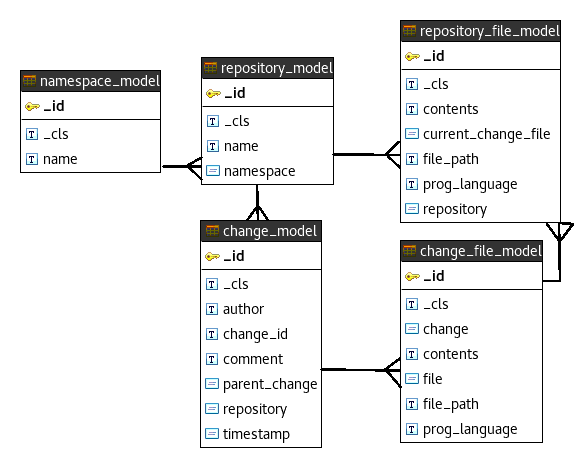
\includegraphics[width=0.75\textwidth]{Figures/nosql-db.png}
    \end{center}
  	\caption{Modelo de Base de Datos en MongoDB.}
    \label{nosql-db}
\end{figure}

El NamespaceModel solo consiste de:
\begin{itemize}
\item el nombre del Namespace
\item el ID que se genera por defecto
\end{itemize}
Esto representa los espacios donde usuarios y grupos pueden crear repositorios. Se considera que los Namespace deben existir de forma única.

El RepositoryModel representa un repositorio y tiene:
\begin{itemize}
\item un nombre
\item permanece a un Namespace
\item el ID que se genera por defecto
\end{itemize}
Cada par de Namespace y Repositorio debe ser una combinación única.

El próximo modelo, RepositoryFileModel, representa un archivo ubicado dentro de un repositorio. Sus atributos son:
\begin{itemize}
\item contenidos del archivo
\item el repositorio a que permanece
\item el lenguaje de programación para que el editor puede cambiar su comportamiento para el lenguaje específico
\item la ubicación del archivo dentro del repositorio incluyendo su nombre
\item un archivo de cambio que representa el estado actual y la última modificación realizada en el mismo, de lo cual se presenta más adelante.
\end{itemize}

El ChangeModel representa un cambio realizado en el repositorio, como los commits de Git. Tiene atributos como:
\begin{itemize}
\item una ID que se lo maneja la aplicación (que viene a ser un hash SHA1, inspirado por Git, de los contenidos y metadatos del mismo cambio)
\item un comentario
\item un autor
\item una estampa de tiempo que tiene tanto la hora como la fecha en que se realizó el cambio
\item el repositorio en que se hizo el cambio
\item una referencia al cambio anterior para que se puede construir una historial de cambios.
\end{itemize}

El ChangeFileModel es como el RepositoryFileModel en que representa archivos, pero en este caso son archivos modificados dentro de un cambio. Por lo tanto lleva los mismos atributos que RepositoryFile solo que en lugar de tener referencias a un repositorio directamente se referencia a un cambio realizado (el cual tiene metadatos como un comentario, autor, cambio previo y momento de modificación) y al archivo del repositorio que modifica (de esta forma puede modificar también la dirección de los archivos quienes no habría otra forma de buscarlos).

Finalmente el TemporaryChangeFileModel no se utiliza actualmente pero como los dos FileModels vistos anteriormente, esta lleva atributos básicos de un archivo. Originalmente se lo planteo para realizar una operación intermedio como la fase del Git Stage en donde se selecciona previo a un commit los cambios que van a estar incluidos dentro del mismo. Pero al final, aunque el modelo de datos esta para suportar varios archivos cambiados dentro de un solo cambio, no esta implementado así. Por temas de tiempo, retraso y alcance, se ha optado por llevar un mini control de versiones de cada archivo dentro de un repositorio, así que en realidad cada cambio en el repositorio solo refleja un archivo cambiado de forma independiente y no hay necesidad para la complejidad del paso intermedio que este modelo representa. 

\index{Controlar Versiones de Código}
\subsubsection{GitLab}
Al settings agregamos las siguientes lineas para configurar la conexión con GitLab:
\lstset{language=Python}
\begin{lstlisting}
GITLAB_DEFAULT_SERVER = '1'

GITLAB_SERVERS = {
    '1': {
        'WITH_TOKEN': True,
        'WITH_CRED': False,
        'API_PROTOCOL': 'http://',
        'API_PORT': '',  # por defecto:
                        # :22 para SSH,
                        # :443 para HTTPS,
                        # :80 para HTTP
        'HOST': '10.10.10.11',
        'SSH_PORT': 22,
        'HTTP_PORT': 80,
        'HTTPS_PORT': 443,
        'USER': "GitEDU",
        'PASSWORD': 'GitEDU2017',
        # expira el 31 de marzo 2018:
        'TOKEN': 'JqMzkgDNvhZ7ofdPa5z5',
        # nunca expira, pero el nivel de 
        # acceso es menor:
        # 'TOKEN': 'TrCfvrdsXzpLFETyc7Q5',  
    }
}
\end{lstlisting}
\lstset{language=Bash}

La conexión a la API de GitLab se realiza de la siguiente manera:
\lstset{language=Python}
\begin{lstlisting}
gitlab_default_srv = GITLAB_DEFAULT_SERVER


def connect_to_gitlab_token(protocol=None,
        host=None, port=None, token=None):
    if host is None:
        return None
    # gitlab_conn = gitlab.Gitlab(protocol
            + host + port, token)
    gitlab_conn = gitlab.Gitlab(protocol
            + host, token)
    #gitlab_conn.auth()
    return gitlab_conn


def connect_to_settings_gitlab_token(
        indx=GITLAB_DEFAULT_SERVER):
    return connect_to_gitlab_token(
            protocol=GITLAB_SERVERS
                [indx]['API_PROTOCOL'],
            host=GITLAB_SERVERS[indx]
                ['HOST'],
            port=GITLAB_SERVERS[indx]
                ['API_PROTOCOL'],
            token=GITLAB_SERVERS[indx]
                ['TOKEN'])


def connect_to_gitlab_user_password(protocol=None,
        host=None, port=None, user=None,
        password=None):
    if host is None:
        return None
    gitlab_conn = gitlab.Gitlab(protocol + host
            + port, email=user, password=password)
    gitlab_conn.auth()
    return gitlab_conn


def connect_to_settings_gitlab_user_password(
        indx=GITLAB_DEFAULT_SERVER):
    return connect_to_gitlab_user_password(
            protocol=GITLAB_SERVERS[indx]
                    ['API_PROTOCOL'],
            host=GITLAB_SERVERS[indx]['HOST'],
            port=GITLAB_SERVERS[indx]
                    ['API_PROTOCOL'],
            user=GITLAB_SERVERS[indx]['USER'],
            password=GITLAB_SERVERS[indx]
                    ['PASSWORD'])


def connect_to_settings_gitlab(
        indx=GITLAB_DEFAULT_SERVER):
    if GITLAB_SERVERS[indx]['WITH_TOKEN']:
        return connect_to_settings_gitlab_token(
                indx)
    elif GITLAB_SERVERS[indx]['WITH_CRED']:
        return connect_to_settings_gitlab_user_password(
                indx)
    else:
        return None

gitlab_srv = None
try:
    gitlab_srv = connect_to_settings_gitlab(
            gitlab_default_srv)
except Exception as e:
    print("No se pudo connectar a GitLab")
    print(e)
\end{lstlisting}
\lstset{language=Bash}

Aunque originalmente se planifico el uso de GitLab como backend de persistencia de codigo (en repositorios, a diferencia de GitEduERP que ocupó snippets), al final no se ocupó el mismo por cinco razones:
\begin{enumerate}
\item La complejidad del API frente documentacion no tan clara del mismo para el community edition (esta mucho mejor documentado el enterprise edition al cual no se tuvo acceso ni en el ambiente de desarollo ni de produccion) y el tiempo disponible.
\item Un gran inestabilidad del servicio.
\item La falta de recursos en los ambientes de produccion y de desarollo que empeora problemas de estabilidad.
\item La simplicidad de utilizar el sistema de ficheros local directamente con GitWeb para hacer el mismo disponible por HTTP.
\item Realmente frente las necesidades actual del proyecto, con tal que no se necesita exponer el servidor de Git a los usuarios finales, no hay necesidad de un servidor de Git de tanta complejidad como el GitLab.
\end{enumerate}
% TODO: maybe this section as an anexo

\subsection{Aspectos Sociales}
Para temas de organización, se ha considerado que aquellos componentes de la aplicación que tienen que ver con interacción social deben existir independientemente de las funcionalidades principales del mismo aplicación. Es con este fin que los componentes del mismo se desarrollaron en un ''app'' distinto 'socialApp'' como fue creada previamente. A futuro se considera el desarollo del mismo para promover interaccion entre estudiantes y tambien otra herramienta de comunicacion e colaboracion entre estudiantes y sus professores que viene a ser un elemento critico para el proceso educativo.

\index{Ejecutar Código}
\section{EduNube}

% TODO: Mandar como anexo:
% TODO: Solo resumir aqui

La gestión de dependencias del sistema EduNube se maneja con un entorno virtual y el gestor de paquetes de python pip. El siguiente es un script de bash diseñado a detectar si es que existe el entorno virtual (lo crea en caso de que no existe) y después instala los requerimientos faltantes como son especificados en un archivo aparte ''requirements.en.txt'' que da librerías y sus versiones.

\begin{lstlisting}
#! /usr/bin/head -n 2
# run with `source activate-en.sh`
PROJECT=en
ENV_DIR=env-$PROJECT
if [ ! -d $ENV_DIR ]; then
        virtualenv --python=python3 $ENV_DIR
fi
source $ENV_DIR/bin/activate
pip3 install -r requirements.$PROJECT.txt
\end{lstlisting}

El script anterior se ejecuta desde el raiz del repositorio con el comando:

\begin{lstlisting}
source activate-en.sh
\end{lstlisting}

Con el entorno creado y activado se puede proceder a instalar cualquier dependencia necesaria que no ha sido instalado previamente:

\begin{lstlisting}
pip3 install django==1.10.6 psycopg2==2.7.1 pymodm==0.4.0\
	ipython
\end{lstlisting}

Para el presente proyecto se instalaron las siguientes dependencias:
\begin{itemize}
	\item Django (1.10.6) como framework para el desarrollo del backend.
    \item Psycopg2 (2.7.1) como librería para conectarse a bases de datos PostgreSQL.
    \item ipython (6.1.0) como interprete interactivo de Python para hacer pruebas en el curso del desarrollo.
\end{itemize}

Con las dependencias instaladas o con cada cambio que se realiza de dependencias se ejecuta el siguiente comando para actualizar la lista de los mismos:

\begin{lstlisting}
pip freeze > requirements.txt
\end{lstlisting}

Se inicia el proyecto de Django con el comando:

\begin{lstlisting}
django-admin startproject EduNube
\end{lstlisting}

También antes de iniciar el desarrollo debe estar configurado el base de datos para ocupar el mismo. Primero es necesario crear y configurar un usuario y base de datos para ser ocupado:

\begin{lstlisting}
su - postgres
psql
\end{lstlisting}
\begin{lstlisting}
	postgres=# CREATE USER edunubeser WITH PASSWORD\
    	'3d?N_6E';
	postgres=# CREATE DATABASE edunubedb WITH OWNER\
    	edunubeser;
	postgres=# \q
psql edunubedb -U postgres
	edunubedb=# CREATE SCHEMA edunubeapp AUTHORIZATION\
    	edunubeser;
	edunubedb=# ALTER USER edunubeser SET search_path\
    	TO edunubeapp;
	edunubedb=# \q
psql edunubedb -U edunubeser
	edunubedb=> SELECT current_schema();
		Debe decir: edunubeapp
	edunubedb=> \q
\end{lstlisting}

Segundo, se abre el settings.py (dentro de la carpeta EduNube/EduNube) y se remplaza (para desarrollo, en producción debe llevar valores distintos) el atributo DATABASES con lo siguiente:
\lstset{language=Python}
\begin{lstlisting}
DATABASES = {
    'default': {
        'ENGINE': 'django.db.backends.postgresql_psycopg2',
        'NAME': 'edunubedb',
        'USER': 'edunubeser',
        'PASSWORD': '3d?N_6E',
        'HOST': '127.0.0.1',
        'PORT': '5432',
    }
}
\end{lstlisting}
\lstset{language=Bash}

Ahora se puede migrar las tablas iniciales de Django:
\begin{lstlisting}
cd EduNube
python manage.py makemigrations
python manage.py migrate
\end{lstlisting}

También creamos un superusuario de Django para temas administrativos:
\begin{lstlisting}
python manage.py createsuperuser
\end{lstlisting}

También se puede crear el app inicial (para lógica del editor de código):
\begin{lstlisting}
python manage.py startapp apiApp
\end{lstlisting}

Y de paso se lo agrega a INSTALLED\_APPS una linea 'apiApp' en el settings.py para que sus tablas definidos a futuro en models.py también se migran con los demás migraciones.

Para resolver un problema de zonas de tiempo, se ha desactivado esta característica de Django con el siguiente linea en el settings.py:
\lstset{language=Python}
\begin{lstlisting}
USE_TZ = False
\end{lstlisting}
\lstset{language=Bash}

Para crear la base de datos de MongoDB:
\begin{lstlisting}
mongo
\end{lstlisting}
\lstset{language=sql}
\begin{lstlisting}
use eduNubeDB
db.createUser(
    {
        user: "eduNubeUser",
        pwd: "3d?N_6E",
        roles: [ "readWrite", "dbAdmin" ]
    }
)
\end{lstlisting}
\lstset{language=Bash}

El mismo se define en el settings de la siguiente manera:
\lstset{language=Python}
\begin{lstlisting}
NOSQL_DATABASES = {
    'nosql': {
        'NAME': 'eduNubeDB',
        'USER': "eduNubeUser",
        'PASSWORD': '3d?N_6E',
        'HOST': '127.0.0.1',
        'PORT': '27017',
    }
}
\end{lstlisting}
\lstset{language=Bash}

\subsection{Autenticación}
El diseño planteado para el sistema EduNube propone dos tipos de autenticación:
\begin{itemize}
\item Clasica para usuarios humanas
\item Basada en Criptografía Asimétrica para ofrecer mayor seguridad y permitir integración con otros sistemas como GitEDU
\end{itemize}

\subsubsection{Autenticación Clasica}
Para la administración del sistema por operador humano se considera necesario la autenticación clásica mediante usuario y contraseña. Para la misma se ocuparon la misma implementación del framework Django y código reutilizado de GitEDU que tiene el mismo propósito.

\subsubsection{Autenticación basado en Criptografía Asimétrica}
Para ofrecer mayor seguridad al sistema de ejecución de código, EduNube, se considera más óptimo utilizar una sistema de autenticación basado en criptografía asimétrica de una manera similar a las llaves de SSH, donde el servidor tiene la oportunidad de conocer bien la identidad del cliente. Aunque no se ha logrado encontrar una implementación factible para la solución planteada, se considera como una solución utilizar una especie de API token similar a otros sistemas. Para generar el token, se ha logrado encontrar un estándar, JSON Web Tokens, que tiene la finalidad de ayudar al servidor identificar y verificar la validez de un cliente desconfiable mediante datos que el servidor mismo cifra con un tipo de llave privada.

A continuación se presenta la lógica para descifrar y cifrar los tokenes con el fin de generar/actualizarlo y también poderlo validar contra una tabla interna de la base de datos a lo que un cliente se lo envía:
\begin{lstlisting}
def decode_api_token(api_token=None):
    if api_token is None:
        raise ValueError("API_Token can't be None")
    return jwt.decode(api_token.token, api_token.secret_key,\
        algorithms=[api_token.token_algo])

def update_api_token(api_token=None, regen_secret_key=False):
    if api_token is None:
        raise ValueError("API_Token can't be None")
    if regen_secret_key or api_token.secret_key is None or\
            len(api_token.secret_key) == 0:
        api_token.secret_key = bcrypt.gensalt()
            # Generate Random Unique Secret_Key
    api_token.edit_date_in_token =\
        api_token.edit_date.__str__()
    payload = {
        'app_name': api_token.app_name,
        'created_date': api_token.created_date.__str__(),
        'edit_date': api_token.edit_date_in_token,
        'expires': api_token.expires
    }
    if api_token.expires:
        if api_token.expire_date is not None:
            payload['expire_date'] = api_token.expire_date
    api_token.token = jwt.encode(payload,\
        api_token.secret_key, algorithm='HS256')\
        # Generate Token
    api_token.save()
\end{lstlisting}

Como parte de la administración de este aspecto del sistema de autenticación, se encuentra implementado las funcionalidades de crear, actualizar, leer y borrar estos tokens de autenticación, siempre y cuando el usuario logueado tenga el permiso ''auth\_admin.manage\_tokens''. Si no se crea este permiso, como es el caso del ambiente de desarrollo, la política de Django es solo permitir cuentas de superusuario para acceder a estas vistas.


\index{Ejecutar Código}
\subsection{Ejecución de Código en Linea}
El de ejecucion de codigo se divide en dos componentes principales que se complementan para dar funcionalidad integra frente las necesidades requeridas. Primero en el sistema de plantillas se define y se controla el ambiente en el cual se ejecuta el codigo y despues en el curso del ciclo de vida del codigo, antes, durante y despues de su ejecuccion se maneja mediante una API externa.

\subsection{Metadatos de Plantillas}
Para ofrecer mayor seguridad y funcionalidad a la ejecucion de codigo en el sistema, se basa en lo que son plantillas de ejecucion diseñados especifcamente para suportar herencia por parte de los usuarios. Estos utilizan varios mecanismos para llegar a este fin, incluyiendo listas negras de archivos que no se puede sobre escribir plantillas que extienden la plantillas (\texttt{.edunubeignore} y\\ \texttt{.edunubeignore.children}), listas blancas de que se debe incluir de archivos cuando recien se crea una nueva plantilla o proyecto en base a la plantilla (.templateinclude), y tokens cifrados para validar repositorios frente un registro centralizado en la base de datos que pertenece al servicio de ejecuccion y tambien la ubicacion del repositorio padre. La herrencia se basa en la creacion de un nuevo repositorio donde se copia uno por uno los contenidos de cada repositorio, desde el inicio de la cadena de herrencia (una plantilla hecha por la administracion para un lenguaje en especifico) hasta el final con el repositorio del usuario, mediante llamadas de \texttt{rsync} y el uso de las listas negras para controlar lo que no se copia en cada fase. De esta forma no se toca la historia original del repositorio del usuario y se puede controlar con mayor facilidad el nivel de control que tiene el usuario final sobre lo que esta ejecutando. 
\subsubsection{.edunubeignore}
El \texttt{.edunubeignore} de un repositorio especifica los archivos de un mismo repositorio que no se deben copiar a sus repositorios hijos, y que tampoco se puede herredar de ningun otro repositorio que le sigue en la herencia de repositorios.
\paragraph{.edunubeignore.children}
El \texttt{.edunubeignore.children} tiene una funcionalidad similar al \texttt{.edunubeignore} pero permite el copia de archivos desde la repositorio actual, pero no de sus repositorios herredetarios.
\subsubsection{.repospec}
El \texttt{.repospec} es un mecanismo que utiliza JWT para dar mayor seguridad de emitir un token que solo puede decifrar el servidor para determinar el repositorio padre de un repositorio. Esto ayuda prevenir ataques contra plantillas de ejecucion en base a la inyeccion de plantillas maliciosas porque realizar un ataque de este tipo requiere que se rompe la cadena de confianza. Este mecanismo todavia se puede mejorar, el cual tema se discuta en trabajos futuros.
\subsubsection{.templateinclude}
El \texttt{.templateinclude} es un archivo de metadatos exclusivo a las plantillas de ejecuccion que determine cual archivos de la plantilla se debe copiar al nuevo repositorio. Esto archivo, combinado con la manera en que el professor realiza el repositorio de la plantilla determina tanto el entorno de ejecucion (donde atraves del mecanismo del \texttt{.edunube}/\texttt{.edunubeignore.children} los archivos que un estudiante no puede sobreescribir de la plantilla) y del estado inicial del proyecto/archivos expuestos al estudiante (atraves del \texttt{.templateinclude}).
% CODE TODO: GitEDU Templates Unimplemented

\subsection{API Externa}
Similar al servicio de GitServerHTTPEndpoint, EduNube tambien ofrece una API externa que requiere un token de autenticacion para su funcionamiento como se lo detalle a continuacion. Ademas se considera critico tres componentes criticos del API:
\begin{enumerate}
  \item API de RepoSpec donde se implementa la creacion y actualizacion de los RepoSpecs de tal forma que al momento de enviar un repositorio a ser ejecutado, se puede validar que el repositorio esta autorizado para ejecucion y de donde previene la herencia del mismo de tal forma que el usuario final no tenga mucho libertad a modificar el mismo y realizar cambios indebidos al entorno de ejecucion.
  \item API de Ejecuccion donde se solita ejecucion de codigo. Esto agrega la solicitud a la cola de trabajo para que el mismo puede ser ejecutado cuando hay disponibilidad.
  \item API de Trabajos (por Lotes) es para soliticar el estado actual de un trabajo y a lo que finaliza, los resultados del mismo trabajo.
\end{enumerate}
\subsubsection{Autenticacion para el API}
Igual que el sistema de GitServerHTTPEndpoint, EduNube utiliza JWT tokens para autorizar y validar llamadas a su API. Estos tokens se los puede administrar usuarios con los permisos adecuados, o por defect (si no se crea los permisos), solo por superusuarios, en el URI \texttt{http://10.10.10.1:8010/auth/tokens}. Dentro de aquello interfaz existe la posibilidad de crear/visualizar tokens \\
(\texttt{http://10.10.10.1:8010/auth/token/<app\_name>.json}), actualizar un token (\texttt{http://10.10.10.1:8010/auth/token/edit/<app\_name>/}), cambiar el secreto (llave privado) de un token\\
(\texttt{http://10.10.10.1:8010/auth/token/secret/<app\_name>/}), y eliminar un token (\texttt{http://10.10.10.1:8010/auth/token/delete/<app\_name>/}).

Para dar conectividad a este servicio desde otro servicio, se copia las respectivas clientes del mismo, llamadas \texttt{execute\_status\_example\_client.py} y \\
\texttt{repospec\_example\_client.py} respectivamente y se agrega las siguientes lineas al settings:
\lstset{language=Python}
\begin{lstlisting}
EDUNUBE_CONFIG = {
    "protocol": "http",
    "host": "10.10.10.1",
    "port": 8010,
    "token": "eyJ0eXAiOiJKV1QiLCJhbGciOiJIUzI1NiJ9.eyJhcHBf"
             "bmFtZSI6IkdpdEVEVSIsImV4cGlyZXMiOmZhbHNlLCJjc"
             "mVhdGVkX2RhdGUiOiIyMDE3LTExLTEyIDE3OjMzOjE3Lj"
             "Y0MTY4MSIsImVkaXRfZGF0ZSI6IjIwMTctMTEtMTIgMjA"
             "6MzY6NDAuMjc5NDAyIn0.825oh2rZUlIPZFaP_UbYPDpd"
             "sXTE0XCaNsia-3NnGuc"
}
\end{lstlisting}

\subsubsection{RepoSpec API}
Los URIs del API de RepoSpecs de EduNube toma la forma general de: \\
\texttt{POST /api/repospec/<operacion>} \\
donde las operaciones posibles son los siguientes:
\begin{itemize}
	\item \texttt{create} para crear un nuevo RepoSpec. Parametros del \texttt{POST} son:
    \begin{description}
    	\item[token] con el API token que generamos previamente.
        \item[repo] con el nombre del repositorio, actualmente no se utiliza este valor, pero a futuro seria de agregarlos a las validaciones de los RepoSpec para prevenir ataques de robo de RepoSpec de un repositorio para otro.
        \item[\textit{parent}] \textit{de forma opcional} con el URI con el cual se puede acceder al repositorio padre del repositorio actual, de aqui parte la herencia de los repositorios y solo en el caso de una repositorio plantilla de ejecuccion que no hereda de ningun otra plantilla, debe ser permitido que este vacio, en cualquier otro caso, incluyendo todos los casos estudiantils, debe ser obligado un valor valido aqui.
    \end{description}
    \item \texttt{get} para leer un RepoSpec existente. Parametros del \texttt{POST} son:
    \begin{description}
    	\item[token] con el API token que generamos previamente.
        \item[\textit{repo}] \textit{de forma opcional} con el nombre del repositorio actual para la busqueda. Dentro de los parametros del \texttt{POST} estar minimo este parametro o el \texttt{repospec\_token}.
        \item[\textit{repospec\_token}] \textit{de forma opcional} con el token del repospec actual para la busqueda. Dentro de los parametros del \texttt{POST} estar minimo este parametro o el \texttt{repo}.
    \end{description}
    \item \texttt{get\_or\_create} para leer un RepoSpec existente o si no existe, crearla. Parametros del \texttt{POST} son:
    \begin{description}
    	\item[token] con el API token que generamos previamente.
        \item[repo] con el nombre del repositorio actual para la busqueda/creacion.
        \item[\textit{parent}] \textit{de forma opcional} con el URI con el cual se puede acceder al repositorio padre del repositorio actual, de aqui parte la herencia de los repositorios y solo en el caso de una repositorio plantilla de ejecuccion que no hereda de ningun otra plantilla, debe ser permitido que este vacio, en cualquier otro caso, incluyendo todos los casos estudiantils, debe ser obligado un valor valido aqui.
        \item[\textit{repospec\_token}] \textit{de forma opcional} con el token del repospec actual para la busqueda.
    \end{description}
    \item \texttt{edit} para modificar un RepoSpec existente. Parametros del \texttt{POST} son:
    \begin{description}
    	\item[token] con el API token que generamos previamente.
        \item[\textit{repo}] \textit{de forma opcional} con el nombre del repositorio actual para la busqueda. Dentro de los parametros del \texttt{POST} estar minimo este parametro o el \texttt{repospec\_token}.
        \item[\textit{repospec\_token}] \textit{de forma opcional} con el token del repospec actual para la busqueda. Dentro de los parametros del \texttt{POST} estar minimo este parametro o el \texttt{repo}.
        \item[\textit{parent}] \textit{de forma opcional} con el URI con el cual se puede acceder al repositorio padre del repositorio actual, de aqui parte la herencia de los repositorios y solo en el caso de una repositorio plantilla de ejecuccion que no hereda de ningun otra plantilla, debe ser permitido que este vacio, en cualquier otro caso, incluyendo todos los casos estudiantils, debe ser obligado un valor valido aqui. Si se deja este sin valor (considerado como Null o en Python None), el comportamiento por defecto es de sobreescribir el valor anterior.
        \item[\textit{new\_repo}] \ldots
        \item[\textit{regen\_secret\_key}] \ldots
    \end{description}
\end{itemize}
% TODO: How to create and modify RepoSpecs via API calls
\subsubsection{Ejecuccion API}
% TODO: How to execute code via API calls
\subsubsection{Jobs API}
% TODO: How to query job state via API calls


%\paragraph{Tokens de Autenticacion}
%Para el uso del API del servicio de GitServerHTTPEndpoint, se emite tokens mediante un interfaz CRUD construido con formularios de Django. Esos API tokens son construidos bajo el estandar JWT o JSON Web Tokens donde el servidor (servicio de Django) generar una llave secreto (mediante la funcion generar sal de bcrypt) y con ello se cifra datos sobre el cliente con el fin de poder validar la identidad del mismo mediante el API token sin que el cliente puede modificar los datos de su API token. El mismo esquema de autenticacion para el API se utiliza con el servicio de EduNube. El acceso al mismo se puede encontrar en el url \url{http://10.10.10.1:8020/auth/tokens} y acceder con cualquier cuenta de superusuario para la creacion, lectura, actualizacion y eliminacion de los API Tokens.
%
%\paragraph{API externa}
%Los URLs del API de GitServerHTTPEndpoint toman la forma general de: 
%\texttt{/api/<tipo\_de\_objeto>/<accion>/<ruta/de/objeto>}\\
%donde los tipos de objetos posibles son
%\begin{itemize}
%	\item \texttt{ns} para los Namespace
%    \item \texttt{repo} para Repositorios y
%    \item \texttt{file} para Archivos
%\end{itemize}
%acciones posibles son:
%\begin{itemize}
%	\item \texttt{create} para crear,
%	\item \texttt{edit} para editar y
%    \item en el caso de los archivos, no existe un solo \texttt{edit} si no una subclasificacion de:
%    \begin{itemize}
%    	\item \texttt{edit/mv}
%        para alterar la ruta de un archivo y 
%        \item \texttt{edit/contents}
%        para alterar los contenidos de un archivo.
%    \end{itemize}
%\end{itemize}
%
%Los URIs del API que operan sobre Namespace, solo acceptan un namespace de parametro con un slash de delimitador final por ejemplo: \\
%\texttt{/api/ns/create/nearley/}
%
%Los URIs del API que opera sobre los repositorios requieren de parametros un namespace y repositorio igual con un slash de delimitador final por ejemplo: \\
%\texttt{/api/repo/create/nearley/GitEDU/}
%
%Los URIs del API que opera sobre archivos toman de parametros un namespace, un repositorio y una ruta de archivos que puede conllevar cualquier numero de slash para indicar directorios dentro del repositorio selecionado, pero la misma ruta no puede terminar en un slash, por ejemplo: \\
%\texttt{/api/file/create/nearley/GitEDU/despliegue/Readme.md}
%
%Un cliente ejemplar de todo el API, se puede encontrar con el nombre \\
%\texttt{example\_client.py} dentro del raiz del proyecto.

